% Options for packages loaded elsewhere
\PassOptionsToPackage{unicode}{hyperref}
\PassOptionsToPackage{hyphens}{url}
\documentclass[
]{article}
\usepackage{xcolor}
\usepackage{amsmath,amssymb}
\setcounter{secnumdepth}{-\maxdimen} % remove section numbering
\usepackage{iftex}
\ifPDFTeX
  \usepackage[T1]{fontenc}
  \usepackage[utf8]{inputenc}
  \usepackage{textcomp} % provide euro and other symbols
\else % if luatex or xetex
  \usepackage{unicode-math} % this also loads fontspec
  \defaultfontfeatures{Scale=MatchLowercase}
  \defaultfontfeatures[\rmfamily]{Ligatures=TeX,Scale=1}
\fi
\usepackage{lmodern}
\ifPDFTeX\else
  % xetex/luatex font selection
\fi
% Use upquote if available, for straight quotes in verbatim environments
\IfFileExists{upquote.sty}{\usepackage{upquote}}{}
\IfFileExists{microtype.sty}{% use microtype if available
  \usepackage[]{microtype}
  \UseMicrotypeSet[protrusion]{basicmath} % disable protrusion for tt fonts
}{}
\makeatletter
\@ifundefined{KOMAClassName}{% if non-KOMA class
  \IfFileExists{parskip.sty}{%
    \usepackage{parskip}
  }{% else
    \setlength{\parindent}{0pt}
    \setlength{\parskip}{6pt plus 2pt minus 1pt}}
}{% if KOMA class
  \KOMAoptions{parskip=half}}
\makeatother
\usepackage{color}
\usepackage{fancyvrb}
\newcommand{\VerbBar}{|}
\newcommand{\VERB}{\Verb[commandchars=\\\{\}]}
\DefineVerbatimEnvironment{Highlighting}{Verbatim}{commandchars=\\\{\}}
% Add ',fontsize=\small' for more characters per line
\newenvironment{Shaded}{}{}
\newcommand{\AlertTok}[1]{\textcolor[rgb]{1.00,0.00,0.00}{\textbf{#1}}}
\newcommand{\AnnotationTok}[1]{\textcolor[rgb]{0.38,0.63,0.69}{\textbf{\textit{#1}}}}
\newcommand{\AttributeTok}[1]{\textcolor[rgb]{0.49,0.56,0.16}{#1}}
\newcommand{\BaseNTok}[1]{\textcolor[rgb]{0.25,0.63,0.44}{#1}}
\newcommand{\BuiltInTok}[1]{\textcolor[rgb]{0.00,0.50,0.00}{#1}}
\newcommand{\CharTok}[1]{\textcolor[rgb]{0.25,0.44,0.63}{#1}}
\newcommand{\CommentTok}[1]{\textcolor[rgb]{0.38,0.63,0.69}{\textit{#1}}}
\newcommand{\CommentVarTok}[1]{\textcolor[rgb]{0.38,0.63,0.69}{\textbf{\textit{#1}}}}
\newcommand{\ConstantTok}[1]{\textcolor[rgb]{0.53,0.00,0.00}{#1}}
\newcommand{\ControlFlowTok}[1]{\textcolor[rgb]{0.00,0.44,0.13}{\textbf{#1}}}
\newcommand{\DataTypeTok}[1]{\textcolor[rgb]{0.56,0.13,0.00}{#1}}
\newcommand{\DecValTok}[1]{\textcolor[rgb]{0.25,0.63,0.44}{#1}}
\newcommand{\DocumentationTok}[1]{\textcolor[rgb]{0.73,0.13,0.13}{\textit{#1}}}
\newcommand{\ErrorTok}[1]{\textcolor[rgb]{1.00,0.00,0.00}{\textbf{#1}}}
\newcommand{\ExtensionTok}[1]{#1}
\newcommand{\FloatTok}[1]{\textcolor[rgb]{0.25,0.63,0.44}{#1}}
\newcommand{\FunctionTok}[1]{\textcolor[rgb]{0.02,0.16,0.49}{#1}}
\newcommand{\ImportTok}[1]{\textcolor[rgb]{0.00,0.50,0.00}{\textbf{#1}}}
\newcommand{\InformationTok}[1]{\textcolor[rgb]{0.38,0.63,0.69}{\textbf{\textit{#1}}}}
\newcommand{\KeywordTok}[1]{\textcolor[rgb]{0.00,0.44,0.13}{\textbf{#1}}}
\newcommand{\NormalTok}[1]{#1}
\newcommand{\OperatorTok}[1]{\textcolor[rgb]{0.40,0.40,0.40}{#1}}
\newcommand{\OtherTok}[1]{\textcolor[rgb]{0.00,0.44,0.13}{#1}}
\newcommand{\PreprocessorTok}[1]{\textcolor[rgb]{0.74,0.48,0.00}{#1}}
\newcommand{\RegionMarkerTok}[1]{#1}
\newcommand{\SpecialCharTok}[1]{\textcolor[rgb]{0.25,0.44,0.63}{#1}}
\newcommand{\SpecialStringTok}[1]{\textcolor[rgb]{0.73,0.40,0.53}{#1}}
\newcommand{\StringTok}[1]{\textcolor[rgb]{0.25,0.44,0.63}{#1}}
\newcommand{\VariableTok}[1]{\textcolor[rgb]{0.10,0.09,0.49}{#1}}
\newcommand{\VerbatimStringTok}[1]{\textcolor[rgb]{0.25,0.44,0.63}{#1}}
\newcommand{\WarningTok}[1]{\textcolor[rgb]{0.38,0.63,0.69}{\textbf{\textit{#1}}}}
\usepackage{longtable,booktabs,array}
\usepackage{caption}
\captionsetup[table]{skip=6pt}
\newcounter{none} % for unnumbered tables
\usepackage{calc} % for calculating minipage widths
% Correct order of tables after \paragraph or \subparagraph
\usepackage{etoolbox}
\makeatletter
\patchcmd\longtable{\par}{\if@noskipsec\mbox{}\fi\par}{}{}
\makeatother
% Allow footnotes in longtable head/foot
\IfFileExists{footnotehyper.sty}{\usepackage{footnotehyper}}{\usepackage{footnote}}
\makesavenoteenv{longtable}
\usepackage{graphicx}
\makeatletter
\newsavebox\pandoc@box
\newcommand*\pandocbounded[1]{% scales image to fit in text height/width
  \sbox\pandoc@box{#1}%
  \Gscale@div\@tempa{\textheight}{\dimexpr\ht\pandoc@box+\dp\pandoc@box\relax}%
  \Gscale@div\@tempb{\linewidth}{\wd\pandoc@box}%
  \ifdim\@tempb\p@<\@tempa\p@\let\@tempa\@tempb\fi% select the smaller of both
  \ifdim\@tempa\p@<\p@\scalebox{\@tempa}{\usebox\pandoc@box}%
  \else\usebox{\pandoc@box}%
  \fi%
}
% Set default figure placement to htbp
\def\fps@figure{htbp}
\makeatother
\setlength{\emergencystretch}{3em} % prevent overfull lines
\providecommand{\tightlist}{%
  \setlength{\itemsep}{0pt}\setlength{\parskip}{0pt}}
\usepackage{bookmark}
\IfFileExists{xurl.sty}{\usepackage{xurl}}{} % add URL line breaks if available
\urlstyle{same}
% fallback for those not using the hyperref driver hyperxmp:
\makeatletter
\@ifundefined{xmpquote}{\newcommand{\xmpquote}[1]{#1}}{}
\makeatother
\hypersetup{
  hidelinks,
  pdfcreator={LaTeX via pandoc}}

\author{}
\date{}

\begin{document}

\protect\phantomsection\label{J0YdC2xdnYx3}
\section{Actividad --- De la web a una
API}\label{actividad--de-la-web-a-una-api}

Bajas estadísticas de equipos de la NHL, entrenas un modelo que predice
si una temporada fue ganadora, y lo dejas respondiendo dentro de un
contenedor.

Al final hay una parte \textbf{opcional}: publicarlo en Internet con una
URL que pueda abrir cualquiera.

\textbf{El código de Python ya está escrito.} Tu trabajo es ejecutarlo,
entender qué pasa en cada paso y responder las preguntas. Lo que sí
tienes que hacer funcionar por tu cuenta es la \textbf{API} y el
\textbf{contenedor}.

\textbf{Entregas:} este notebook ejecutado + una captura de la API
respondiendo.

\protect\phantomsection\label{5TGWXZjUnYx-}
\begin{center}\rule{0.5\linewidth}{0.5pt}\end{center}

\subsection{Antes de empezar: ¿qué vamos a
predecir?}\label{antes-de-empezar-quuxe9-vamos-a-predecir}

Cada fila de los datos son \textbf{las estadísticas de un equipo de la
NHL en una temporada}. El scraper construye estas nueve columnas:

\begin{Shaded}
\begin{Highlighting}[]
\NormalTok{COLS }\OperatorTok{=}\NormalTok{ [}\StringTok{"equipo"}\NormalTok{, }\StringTok{"anio"}\NormalTok{, }\StringTok{"victorias"}\NormalTok{, }\StringTok{"derrotas"}\NormalTok{, }\StringTok{"ot"}\NormalTok{,}
        \StringTok{"win\_pct"}\NormalTok{, }\StringTok{"gf"}\NormalTok{, }\StringTok{"ga"}\NormalTok{, }\StringTok{"dif"}\NormalTok{]}
\end{Highlighting}
\end{Shaded}

Las cuatro que importan hoy:

{\def\LTcaptype{none} % do not increment counter
\begin{longtable}[]{@{}ll@{}}
\toprule\noalign{}
columna & qué es \\
\midrule\noalign{}
\endhead
\bottomrule\noalign{}
\endlastfoot
\texttt{gf} & \emph{goals for} --- goles que \textbf{anotó} el equipo \\
\texttt{ga} & \emph{goals against} --- goles que \textbf{recibió} \\
\texttt{dif} & la diferencia: \texttt{gf\ -\ ga} \\
\texttt{win\_pct} & la proporción de partidos ganados \\
\end{longtable}
}

Así se ve, en concreto:

\begin{verbatim}
equipo     gf    ga    dif    win_pct
Boston     300   220     80      0.67
Detroit    210   280    -70      0.38
\end{verbatim}

Boston anotó 80 goles más de los que recibió y ganó el 67 \% de sus
partidos. Detroit recibió 70 más de los que anotó y ganó el 38 \%.

\textbf{La pregunta que va a responder el modelo:}

\begin{quote}
Sabiendo cuántos goles anotó un equipo y cuántos recibió, ¿su temporada
fue \textbf{ganadora}?
\end{quote}

Un detalle importante: la respuesta (\emph{ganadora} sí o no) \textbf{no
viene en la tabla}. La vamos a construir nosotros en la parte 2.

\protect\phantomsection\label{0pRQ7sVjnYyB}
\begin{center}\rule{0.5\linewidth}{0.5pt}\end{center}

\subsection{0 · Las librerías}\label{0--las-libreruxedas}

Ejecuta esta celda una vez. \texttt{pyarrow} es el motor que necesita
Pandas para escribir archivos \textbf{Parquet}; sin él, el
\texttt{to\_parquet} de la parte 1 falla.

\protect\phantomsection\label{l2ew8ZjinYyB}
\begin{Shaded}
\begin{Highlighting}[]
\CommentTok{\# se ejecuta una sola vez; si ya están instaladas, no hace nada}
\OperatorTok{\%}\NormalTok{pip install }\OperatorTok{{-}}\NormalTok{q requests beautifulsoup4 pandas pyarrow scikit}\OperatorTok{{-}}\NormalTok{learn joblib matplotlib}
\end{Highlighting}
\end{Shaded}

\begin{verbatim}
Note: you may need to restart the kernel to use updated packages.
\end{verbatim}

\protect\phantomsection\label{9CNEWlc3nYyD}
\begin{center}\rule{0.5\linewidth}{0.5pt}\end{center}

\subsection{1 · Bajar los datos}\label{1--bajar-los-datos}

La página muestra 100 equipos por vez y se pagina con
\texttt{?page\_num=}. Primero probamos \textbf{una} página.

\protect\phantomsection\label{I9i3q27KnYyF}
\begin{Shaded}
\begin{Highlighting}[]
\ImportTok{import}\NormalTok{ time}
\ImportTok{import}\NormalTok{ requests}
\ImportTok{import}\NormalTok{ pandas }\ImportTok{as}\NormalTok{ pd}
\ImportTok{from}\NormalTok{ bs4 }\ImportTok{import}\NormalTok{ BeautifulSoup}

\NormalTok{URL }\OperatorTok{=} \StringTok{"https://www.scrapethissite.com/pages/forms/?page\_num=}\SpecialCharTok{\{\}}\StringTok{\&per\_page=100"}
\NormalTok{COLS }\OperatorTok{=}\NormalTok{ [}\StringTok{"equipo"}\NormalTok{, }\StringTok{"anio"}\NormalTok{, }\StringTok{"victorias"}\NormalTok{, }\StringTok{"derrotas"}\NormalTok{, }\StringTok{"ot"}\NormalTok{, }\StringTok{"win\_pct"}\NormalTok{,}
        \StringTok{"gf"}\NormalTok{, }\StringTok{"ga"}\NormalTok{, }\StringTok{"dif"}\NormalTok{]}

\KeywordTok{def}\NormalTok{ leer\_pagina(n):}
    \CommentTok{"""Devuelve las filas de una página como lista de diccionarios."""}
\NormalTok{    sopa }\OperatorTok{=}\NormalTok{ BeautifulSoup(requests.get(URL.}\BuiltInTok{format}\NormalTok{(n), timeout}\OperatorTok{=}\DecValTok{20}\NormalTok{).text,}
                         \StringTok{"html.parser"}\NormalTok{)}
\NormalTok{    filas }\OperatorTok{=}\NormalTok{ []}
    \ControlFlowTok{for}\NormalTok{ tr }\KeywordTok{in}\NormalTok{ sopa.select(}\StringTok{"tr.team"}\NormalTok{):                 }\CommentTok{\# ← el selector CSS}
\NormalTok{        celdas }\OperatorTok{=}\NormalTok{ [td.text.strip() }\ControlFlowTok{for}\NormalTok{ td }\KeywordTok{in}\NormalTok{ tr.select(}\StringTok{"td"}\NormalTok{)]}
\NormalTok{        filas.append(}\BuiltInTok{dict}\NormalTok{(}\BuiltInTok{zip}\NormalTok{(COLS, celdas)))}
    \ControlFlowTok{return}\NormalTok{ filas}

\BuiltInTok{print}\NormalTok{(}\BuiltInTok{len}\NormalTok{(leer\_pagina(}\DecValTok{1}\NormalTok{)), }\StringTok{"filas en la página 1"}\NormalTok{)}
\end{Highlighting}
\end{Shaded}

\begin{verbatim}
100 filas en la página 1
\end{verbatim}

\protect\phantomsection\label{XT2pqa_fnYyG}
Ahora las seis.

\begin{quote}
\textbf{Si la página no responde} (se cayó el sitio, la red la bloquea,
cambió el HTML): no pierdas la mañana. En el aula virtual está
\textbf{\texttt{equipos\_respaldo.csv}} con las mismas 582 filas. Súbelo
a esta carpeta y usa esta línea en lugar de la celda de abajo:

\begin{Shaded}
\begin{Highlighting}[]
\NormalTok{equipos }\OperatorTok{=}\NormalTok{ pd.read\_csv(}\StringTok{"equipos\_respaldo.csv"}\NormalTok{)}
\end{Highlighting}
\end{Shaded}

Todo lo que sigue funciona igual.
\end{quote}

\protect\phantomsection\label{2_JbUPbMnYyH}
\begin{Shaded}
\begin{Highlighting}[]
\NormalTok{datos }\OperatorTok{=}\NormalTok{ []}

\ControlFlowTok{for}\NormalTok{ n }\KeywordTok{in} \BuiltInTok{range}\NormalTok{(}\DecValTok{1}\NormalTok{, }\DecValTok{7}\NormalTok{):            }\CommentTok{\# 6 páginas × 100 filas}
\NormalTok{    datos }\OperatorTok{+=}\NormalTok{ leer\_pagina(n)}
    \BuiltInTok{print}\NormalTok{(}\SpecialStringTok{f"página }\SpecialCharTok{\{}\NormalTok{n}\SpecialCharTok{\}}\SpecialStringTok{"}\NormalTok{, end}\OperatorTok{=}\StringTok{"  "}\NormalTok{)}
\NormalTok{    time.sleep(}\FloatTok{0.5}\NormalTok{)              }\CommentTok{\# educación: una pausa entre pedidos}

\BuiltInTok{print}\NormalTok{(}\StringTok{"}\CharTok{\textbackslash{}n}\StringTok{"}\NormalTok{, }\BuiltInTok{len}\NormalTok{(datos), }\StringTok{"filas"}\NormalTok{)}
\end{Highlighting}
\end{Shaded}

\begin{verbatim}
página 1  página 2  página 3  página 4  página 5  página 6  
 582 filas
\end{verbatim}

\protect\phantomsection\label{CstpQk21nYyI}
Lo que llega de la web es \textbf{texto}: \texttt{"44"} no es el número
44. Hay que convertirlo antes de poder calcular nada.

Guardamos el resultado en los dos formatos que vimos esta semana, para
compararlos.

\protect\phantomsection\label{GcmKL8mNnYyL}
\begin{Shaded}
\begin{Highlighting}[]
\NormalTok{equipos }\OperatorTok{=}\NormalTok{ pd.DataFrame(datos)}

\CommentTok{\# lo que llega de la web es TEXTO: hay que convertirlo a número}
\ControlFlowTok{for}\NormalTok{ c }\KeywordTok{in}\NormalTok{ [}\StringTok{"anio"}\NormalTok{, }\StringTok{"victorias"}\NormalTok{, }\StringTok{"derrotas"}\NormalTok{, }\StringTok{"gf"}\NormalTok{, }\StringTok{"ga"}\NormalTok{, }\StringTok{"dif"}\NormalTok{]:}
\NormalTok{    equipos[c] }\OperatorTok{=}\NormalTok{ pd.to\_numeric(equipos[c], errors}\OperatorTok{=}\StringTok{"coerce"}\NormalTok{)}
\NormalTok{equipos[}\StringTok{"win\_pct"}\NormalTok{] }\OperatorTok{=}\NormalTok{ pd.to\_numeric(equipos[}\StringTok{"win\_pct"}\NormalTok{], errors}\OperatorTok{=}\StringTok{"coerce"}\NormalTok{)}

\NormalTok{equipos.to\_csv(}\StringTok{"equipos.csv"}\NormalTok{, index}\OperatorTok{=}\VariableTok{False}\NormalTok{)}
\NormalTok{equipos.to\_parquet(}\StringTok{"equipos.parquet"}\NormalTok{, index}\OperatorTok{=}\VariableTok{False}\NormalTok{)   }\CommentTok{\# necesita pyarrow}

\ImportTok{import}\NormalTok{ os}
\BuiltInTok{print}\NormalTok{(}\SpecialStringTok{f"csv     }\SpecialCharTok{\{}\NormalTok{os}\SpecialCharTok{.}\NormalTok{path}\SpecialCharTok{.}\NormalTok{getsize(}\StringTok{\textquotesingle{}equipos.csv\textquotesingle{}}\NormalTok{)}\OperatorTok{/}\DecValTok{1024}\SpecialCharTok{:6.1f\}}\SpecialStringTok{ KB"}\NormalTok{)}
\BuiltInTok{print}\NormalTok{(}\SpecialStringTok{f"parquet }\SpecialCharTok{\{}\NormalTok{os}\SpecialCharTok{.}\NormalTok{path}\SpecialCharTok{.}\NormalTok{getsize(}\StringTok{\textquotesingle{}equipos.parquet\textquotesingle{}}\NormalTok{)}\OperatorTok{/}\DecValTok{1024}\SpecialCharTok{:6.1f\}}\SpecialStringTok{ KB"}\NormalTok{)}
\NormalTok{equipos.head(}\DecValTok{3}\NormalTok{)}
\end{Highlighting}
\end{Shaded}

\begin{verbatim}
csv       27.1 KB
parquet   12.7 KB
\end{verbatim}

\begin{verbatim}
           equipo  anio  victorias  derrotas ot  win_pct   gf   ga  dif
0   Boston Bruins  1990         44        24       0.550  299  264   35
1  Buffalo Sabres  1990         31        30       0.388  292  278   14
2  Calgary Flames  1990         46        26       0.575  344  263   81
\end{verbatim}

\protect\phantomsection\label{DxpAXQk-nYyL}
\begin{quote}
\textbf{Anota} los dos tamaños. ¿Te sorprende cuál gana?
\end{quote}

\textbf{Respuesta:}: Los equipos canadienses son mas naturales para
jugar hockey que en los EE.UU.

\protect\phantomsection\label{qzM2isTEnYyN}
\begin{center}\rule{0.5\linewidth}{0.5pt}\end{center}

\subsection{2 · La variable objetivo}\label{2--la-variable-objetivo}

Los datos no traen una columna que diga «esta temporada fue buena». La
creamos nosotros a partir de \texttt{win\_pct}, con una regla sencilla:

\[
\text{ganadora} =
\begin{cases}
\text{True}, & \text{si } win\_pct > 0.5 \\
\text{False}, & \text{si } win\_pct \le 0.5
\end{cases}
\]

En ejemplos:

\begin{verbatim}
win_pct = 0.65  ->  ganadora = True
win_pct = 0.54  ->  ganadora = True
win_pct = 0.50  ->  ganadora = False     ← ojo
win_pct = 0.42  ->  ganadora = False
\end{verbatim}

\textbf{Fíjate en el tercero.} Usamos \texttt{\textgreater{}\ 0.5}, no
\texttt{\textgreater{}=\ 0.5}. Una temporada con exactamente la mitad de
partidos ganados \textbf{no} cuenta como ganadora. Es una decisión
nuestra, y podría haber sido la contraria: así de concretas son las
definiciones en un problema real.

A esta columna se la llama \textbf{variable objetivo} (o \emph{target},
o \emph{etiqueta}): es lo que queremos que el modelo aprenda a predecir.

\protect\phantomsection\label{ImBdBYyynYyN}
\begin{Shaded}
\begin{Highlighting}[]
\NormalTok{equipos[}\StringTok{"ganadora"}\NormalTok{] }\OperatorTok{=}\NormalTok{ equipos[}\StringTok{"win\_pct"}\NormalTok{] }\OperatorTok{\textgreater{}} \FloatTok{0.5}

\NormalTok{equipos[[}\StringTok{"equipo"}\NormalTok{, }\StringTok{"anio"}\NormalTok{, }\StringTok{"gf"}\NormalTok{, }\StringTok{"ga"}\NormalTok{, }\StringTok{"dif"}\NormalTok{, }\StringTok{"win\_pct"}\NormalTok{, }\StringTok{"ganadora"}\NormalTok{]].head()}
\end{Highlighting}
\end{Shaded}

\begin{verbatim}
               equipo  anio   gf   ga  dif  win_pct  ganadora
0       Boston Bruins  1990  299  264   35    0.550      True
1      Buffalo Sabres  1990  292  278   14    0.388     False
2      Calgary Flames  1990  344  263   81    0.575      True
3  Chicago Blackhawks  1990  284  211   73    0.613      True
4   Detroit Red Wings  1990  273  298  -25    0.425     False
\end{verbatim}

\protect\phantomsection\label{C-e9HEOAnYyO}
Ahora veamos \textbf{cuántas temporadas hay de cada tipo}.

\texttt{value\_counts(normalize=True)} cuenta cuántas filas hay de cada
valor y lo convierte en proporción. Si sale algo como:

\begin{verbatim}
False    0.71
True     0.29
\end{verbatim}

significa que el \textbf{71 \% de las temporadas no fueron ganadoras} y
el \textbf{29 \% sí}.

Dos aclaraciones que evitan confusiones:

\begin{itemize}
\tightlist
\item
  Esos números \textbf{no son predicciones de ningún modelo}. Todavía no
  hemos entrenado nada. Es simplemente cómo están repartidos los datos.
\item
  Como no están cerca de 50 \% y 50 \%, decimos que las clases están
  \textbf{desbalanceadas}. Recuerda ese detalle: va a ser importante en
  un rato.
\end{itemize}

La segunda tabla muestra la diferencia media de goles en cada grupo. Si
los dos números son muy distintos, es buena señal: significa que
\texttt{dif} \textbf{sí} distingue los dos tipos de temporada.

\protect\phantomsection\label{ceplGF5TnYyP}
\begin{Shaded}
\begin{Highlighting}[]
\BuiltInTok{print}\NormalTok{(equipos[}\StringTok{"ganadora"}\NormalTok{].value\_counts(normalize}\OperatorTok{=}\VariableTok{True}\NormalTok{).}\BuiltInTok{round}\NormalTok{(}\DecValTok{2}\NormalTok{))}
\BuiltInTok{print}\NormalTok{()}
\BuiltInTok{print}\NormalTok{(}\StringTok{"diferencia media de goles en cada grupo:"}\NormalTok{)}
\BuiltInTok{print}\NormalTok{(equipos.groupby(}\StringTok{"ganadora"}\NormalTok{)[}\StringTok{"dif"}\NormalTok{].mean().}\BuiltInTok{round}\NormalTok{(}\DecValTok{1}\NormalTok{))}
\end{Highlighting}
\end{Shaded}

\begin{verbatim}
ganadora
False    0.65
True     0.35
Name: proportion, dtype: float64

diferencia media de goles en cada grupo:
ganadora
False   -21.3
True     40.2
Name: dif, dtype: float64
\end{verbatim}

\protect\phantomsection\label{zqsjgHc7nYyP}
\begin{center}\rule{0.5\linewidth}{0.5pt}\end{center}

\subsection{\texorpdfstring{3 · \texttt{X} e \texttt{y}: lo que ve el
modelo y lo que debe
adivinar}{3 · X e y: lo que ve el modelo y lo que debe adivinar}}\label{3--x-e-y-lo-que-ve-el-modelo-y-lo-que-debe-adivinar}

Para entrenar cualquier modelo hay que separar los datos en dos cosas.

\subsubsection{\texorpdfstring{\texttt{X} --- las características
(\emph{features})}{X --- las características (features)}}\label{x--las-caracteruxedsticas-features}

Son las columnas que el modelo \textbf{puede mirar} para decidir:

\begin{verbatim}
X

gf    ga    dif
300   250    50
210   270   -60
280   260    20
\end{verbatim}

\begin{itemize}
\tightlist
\item
  cada \textbf{fila} es la temporada de un equipo
\item
  cada \textbf{columna} es una característica
\end{itemize}

Si hay \texttt{n} temporadas, \texttt{X} tiene forma \(n \times 3\):
\texttt{n} filas y 3 características.

\subsubsection{\texorpdfstring{\texttt{y} --- la variable objetivo
(\emph{target})}{y --- la variable objetivo (target)}}\label{y--la-variable-objetivo-target}

Es la respuesta correcta de cada fila:

\begin{verbatim}
y

True
False
True
\end{verbatim}

\subsubsection{Cómo se relacionan}\label{cuxf3mo-se-relacionan}

Cada fila de \texttt{X} tiene su respuesta en \texttt{y}, en la misma
posición:

\begin{verbatim}
gf    ga    dif        ganadora
300   250    50   ->     True
210   270   -60   ->     False
280   260    20   ->     True
\end{verbatim}

Eso es el \textbf{aprendizaje supervisado}: darle al modelo muchos pares
\emph{(pregunta, respuesta)} para que encuentre la relación

\[X \longrightarrow y\]

o dicho en palabras:

\begin{verbatim}
[goles a favor, goles en contra, diferencia]
                    ↓
              ¿ganadora o no?
\end{verbatim}

\protect\phantomsection\label{nVa_K6jXnYyQ}
\begin{Shaded}
\begin{Highlighting}[]
\NormalTok{X }\OperatorTok{=}\NormalTok{ equipos[[}\StringTok{"gf"}\NormalTok{, }\StringTok{"ga"}\NormalTok{, }\StringTok{"dif"}\NormalTok{]]    }\CommentTok{\# lo que el modelo VE}
\NormalTok{y }\OperatorTok{=}\NormalTok{ equipos[}\StringTok{"ganadora"}\NormalTok{]             }\CommentTok{\# lo que el modelo debe ADIVINAR}

\BuiltInTok{print}\NormalTok{(}\StringTok{"X:"}\NormalTok{, X.shape, }\StringTok{" {-}\textgreater{} (filas, características)"}\NormalTok{)}
\BuiltInTok{print}\NormalTok{(}\StringTok{"y:"}\NormalTok{, y.shape)}
\NormalTok{X.head(}\DecValTok{3}\NormalTok{)}
\end{Highlighting}
\end{Shaded}

\begin{verbatim}
X: (582, 3)  -> (filas, características)
y: (582,)
\end{verbatim}

\begin{verbatim}
    gf   ga  dif
0  299  264   35
1  292  278   14
2  344  263   81
\end{verbatim}

\protect\phantomsection\label{Gxj2l4cfnYyR}
Y ahora partimos los datos en dos:

\begin{itemize}
\tightlist
\item
  \textbf{entrenamiento (70 \%)} --- el modelo los estudia
\item
  \textbf{prueba (30 \%)} --- el modelo \textbf{nunca} los ve durante el
  entrenamiento; sirven para medir si de verdad aprendió o solo memorizó
\end{itemize}

\texttt{stratify=y} mantiene la misma proporción de ganadoras en los dos
grupos. Sin eso, por azar, el grupo de prueba podría quedar con muy
pocas.

\protect\phantomsection\label{SoeK6j6PnYyS}
\begin{Shaded}
\begin{Highlighting}[]
\ImportTok{from}\NormalTok{ sklearn.model\_selection }\ImportTok{import}\NormalTok{ train\_test\_split}

\NormalTok{X\_tr, X\_te, y\_tr, y\_te }\OperatorTok{=}\NormalTok{ train\_test\_split(}
\NormalTok{    X, y, test\_size}\OperatorTok{=}\FloatTok{0.3}\NormalTok{, stratify}\OperatorTok{=}\NormalTok{y, random\_state}\OperatorTok{=}\DecValTok{0}\NormalTok{)}

\BuiltInTok{print}\NormalTok{(}\SpecialStringTok{f"entrenamiento: }\SpecialCharTok{\{}\BuiltInTok{len}\NormalTok{(X\_tr)}\SpecialCharTok{\}}\SpecialStringTok{ filas"}\NormalTok{)}
\BuiltInTok{print}\NormalTok{(}\SpecialStringTok{f"prueba:        }\SpecialCharTok{\{}\BuiltInTok{len}\NormalTok{(X\_te)}\SpecialCharTok{\}}\SpecialStringTok{ filas"}\NormalTok{)}
\end{Highlighting}
\end{Shaded}

\begin{verbatim}
entrenamiento: 407 filas
prueba:        175 filas
\end{verbatim}

\protect\phantomsection\label{OwgEQubunYyS}
\begin{center}\rule{0.5\linewidth}{0.5pt}\end{center}

\subsection{4 · Primero, el modelo
tonto}\label{4--primero-el-modelo-tonto}

Antes de entrenar nada serio, necesitamos saber \textbf{contra qué
comparar}. A ese punto de referencia se le llama \textbf{baseline}.

\texttt{DummyClassifier(strategy="most\_frequent")} hace lo más simple
imaginable: mira cuál es la clase más frecuente en el entrenamiento y
\textbf{responde siempre esa}, sin mirar \texttt{gf}, \texttt{ga} ni
\texttt{dif}.

Si la mayoría de las temporadas son perdedoras, el modelo tonto
responde:

\begin{verbatim}
False
False
False
False
...
\end{verbatim}

Y acierta bastante, solo por repetir la respuesta más común:

\begin{verbatim}
Real       Predicción del tonto
False      False   ✓
False      False   ✓
True       False   ✗
False      False   ✓
True       False   ✗
\end{verbatim}

\textbf{Para qué sirve esto.} Antes de decir «mi modelo tiene 90 \% de
exactitud», hay que responder: \emph{¿es mejor que esta estrategia que
ni siquiera mira los datos?} Si tu modelo saca 0.67 y el tonto saca
0.65, no has construido nada.

\begin{quote}
Un modelo útil tiene que ganarle al baseline \textbf{por un margen
claro}.
\end{quote}

\protect\phantomsection\label{i0ELhWl4nYyT}
\begin{Shaded}
\begin{Highlighting}[]
\ImportTok{from}\NormalTok{ sklearn.dummy }\ImportTok{import}\NormalTok{ DummyClassifier}
\ImportTok{from}\NormalTok{ sklearn.metrics }\ImportTok{import}\NormalTok{ accuracy\_score, f1\_score}

\NormalTok{tonto }\OperatorTok{=}\NormalTok{ DummyClassifier(strategy}\OperatorTok{=}\StringTok{"most\_frequent"}\NormalTok{).fit(X\_tr, y\_tr)}
\NormalTok{p }\OperatorTok{=}\NormalTok{ tonto.predict(X\_te)}

\BuiltInTok{print}\NormalTok{(}\StringTok{"sus 5 primeras predicciones:"}\NormalTok{, p[:}\DecValTok{5}\NormalTok{])}
\BuiltInTok{print}\NormalTok{(}\SpecialStringTok{f"MODELO TONTO   exactitud }\SpecialCharTok{\{}\NormalTok{accuracy\_score(y\_te, p)}\SpecialCharTok{:.3f\}}\SpecialStringTok{"}
      \SpecialStringTok{f"   F1 }\SpecialCharTok{\{}\NormalTok{f1\_score(y\_te, p)}\SpecialCharTok{:.3f\}}\SpecialStringTok{"}\NormalTok{)}
\end{Highlighting}
\end{Shaded}

\begin{verbatim}
sus 5 primeras predicciones: [False False False False False]
MODELO TONTO   exactitud 0.651   F1 0.000
\end{verbatim}

\protect\phantomsection\label{4ATkp7rpnYyU}
\begin{quote}
\textbf{Anota ese número.} Es el que tu modelo tiene que superar.
\end{quote}

\protect\phantomsection\label{G4sSjVFsnYyU}
\begin{center}\rule{0.5\linewidth}{0.5pt}\end{center}

\subsection{5 · Entrenar el modelo de
verdad}\label{5--entrenar-el-modelo-de-verdad}

Usamos un \textbf{Pipeline} con dos pasos:

\begin{enumerate}
\tightlist
\item
  \texttt{StandardScaler} --- pone las tres columnas en la misma escala
\item
  \texttt{LogisticRegression} --- el clasificador
\end{enumerate}

Guardarlos juntos importa: cuando el modelo salga a producir
predicciones, los datos nuevos tendrán que pasar por
\textbf{exactamente} las mismas transformaciones.

\protect\phantomsection\label{9-rFH6SAnYyV}
\begin{Shaded}
\begin{Highlighting}[]
\ImportTok{from}\NormalTok{ sklearn.pipeline }\ImportTok{import}\NormalTok{ make\_pipeline}
\ImportTok{from}\NormalTok{ sklearn.preprocessing }\ImportTok{import}\NormalTok{ StandardScaler}
\ImportTok{from}\NormalTok{ sklearn.linear\_model }\ImportTok{import}\NormalTok{ LogisticRegression}

\NormalTok{modelo }\OperatorTok{=}\NormalTok{ make\_pipeline(StandardScaler(), LogisticRegression(max\_iter}\OperatorTok{=}\DecValTok{5000}\NormalTok{))}
\NormalTok{modelo.fit(X\_tr, y\_tr)}

\NormalTok{pred }\OperatorTok{=}\NormalTok{ modelo.predict(X\_te)}
\BuiltInTok{print}\NormalTok{(}\SpecialStringTok{f"TU MODELO      exactitud }\SpecialCharTok{\{}\NormalTok{accuracy\_score(y\_te, pred)}\SpecialCharTok{:.3f\}}\SpecialStringTok{"}
      \SpecialStringTok{f"   F1 }\SpecialCharTok{\{}\NormalTok{f1\_score(y\_te, pred)}\SpecialCharTok{:.3f\}}\SpecialStringTok{"}\NormalTok{)}
\end{Highlighting}
\end{Shaded}

\begin{verbatim}
TU MODELO      exactitud 0.811   F1 0.723
\end{verbatim}

\protect\phantomsection\label{POMYtmSunYyV}
Compara los resultados con los del modelo tonto. Mira \textbf{tanto la
exactitud como el F1}, porque las dos métricas no cuentan exactamente la
misma historia.

\subsubsection{Qué miden precision, recall y
F1}\label{quuxe9-miden-precision-recall-y-f1}

Nos centramos en la clase que nos interesa detectar:
\texttt{ganadora\ =\ True}.

\textbf{Precisión} --- de todas las que el modelo \emph{dijo} que eran
ganadoras, ¿cuántas lo eran de verdad?

\[Precision = \frac{TP}{TP + FP}\]

\textbf{Recall} --- de todas las que \emph{realmente} eran ganadoras,
¿cuántas encontró?

\[Recall = \frac{TP}{TP + FN}\]

\textbf{F1} --- combina las dos en un solo número:

\[F1 = 2 \cdot \frac{Precision \cdot Recall}{Precision + Recall}\]

Lo único que hay que recordar de esa fórmula: \textbf{el F1 solo es alto
si las dos son altas}. Si una de las dos se hunde, el F1 se hunde con
ella.

\subsubsection{Por qué esto importa con el modelo
tonto}\label{por-quuxe9-esto-importa-con-el-modelo-tonto}

Si el modelo tonto nunca dice \texttt{True}, no encuentra
\textbf{ninguna} temporada ganadora: su recall para esa clase es 0, y
por lo tanto su F1 también es 0 --- por muy alta que sea su exactitud.

\begin{quote}
\textbf{La exactitud puede esconder que un modelo ignora por completo
una de las clases. El F1 lo deja a la vista.}
\end{quote}

Un detalle técnico de la celda siguiente: \texttt{zero\_division=0}
evita un aviso de \texttt{scikit-learn} cuando un modelo no predice
ningún ejemplo de una clase. En ese caso la precisión sería una división
por cero, y con este parámetro se reporta como 0 en lugar de lanzar un
warning. Puede pasar justamente con el modelo tonto.

\protect\phantomsection\label{8Vv7XwwqnYyW}
\begin{Shaded}
\begin{Highlighting}[]
\ImportTok{from}\NormalTok{ sklearn.metrics }\ImportTok{import}\NormalTok{ classification\_report, ConfusionMatrixDisplay}
\ImportTok{import}\NormalTok{ matplotlib.pyplot }\ImportTok{as}\NormalTok{ plt}

\BuiltInTok{print}\NormalTok{(}\StringTok{"{-}{-}{-} MODELO TONTO"}\NormalTok{)}
\BuiltInTok{print}\NormalTok{(classification\_report(y\_te, p, zero\_division}\OperatorTok{=}\DecValTok{0}\NormalTok{))}

\BuiltInTok{print}\NormalTok{(}\StringTok{"{-}{-}{-} TU MODELO"}\NormalTok{)}
\BuiltInTok{print}\NormalTok{(classification\_report(y\_te, pred, zero\_division}\OperatorTok{=}\DecValTok{0}\NormalTok{))}

\NormalTok{fig, axes }\OperatorTok{=}\NormalTok{ plt.subplots(}\DecValTok{1}\NormalTok{, }\DecValTok{2}\NormalTok{, figsize}\OperatorTok{=}\NormalTok{(}\DecValTok{10}\NormalTok{, }\DecValTok{4}\NormalTok{))}

\NormalTok{ConfusionMatrixDisplay.from\_estimator(}
\NormalTok{    tonto, X\_te, y\_te, display\_labels}\OperatorTok{=}\NormalTok{[}\StringTok{"perdedora"}\NormalTok{, }\StringTok{"ganadora"}\NormalTok{], ax}\OperatorTok{=}\NormalTok{axes[}\DecValTok{0}\NormalTok{])}
\NormalTok{axes[}\DecValTok{0}\NormalTok{].set\_title(}\StringTok{"Modelo tonto"}\NormalTok{)}

\NormalTok{ConfusionMatrixDisplay.from\_estimator(}
\NormalTok{    modelo, X\_te, y\_te, display\_labels}\OperatorTok{=}\NormalTok{[}\StringTok{"perdedora"}\NormalTok{, }\StringTok{"ganadora"}\NormalTok{], ax}\OperatorTok{=}\NormalTok{axes[}\DecValTok{1}\NormalTok{])}
\NormalTok{axes[}\DecValTok{1}\NormalTok{].set\_title(}\StringTok{"Tu modelo"}\NormalTok{)}

\NormalTok{plt.tight\_layout()}
\NormalTok{plt.show()}
\end{Highlighting}
\end{Shaded}

\begin{verbatim}
--- MODELO TONTO
              precision    recall  f1-score   support

       False       0.65      1.00      0.79       114
        True       0.00      0.00      0.00        61

    accuracy                           0.65       175
   macro avg       0.33      0.50      0.39       175
weighted avg       0.42      0.65      0.51       175

--- TU MODELO
              precision    recall  f1-score   support

       False       0.85      0.87      0.86       114
        True       0.74      0.70      0.72        61

    accuracy                           0.81       175
   macro avg       0.79      0.79      0.79       175
weighted avg       0.81      0.81      0.81       175

\end{verbatim}

\pandocbounded{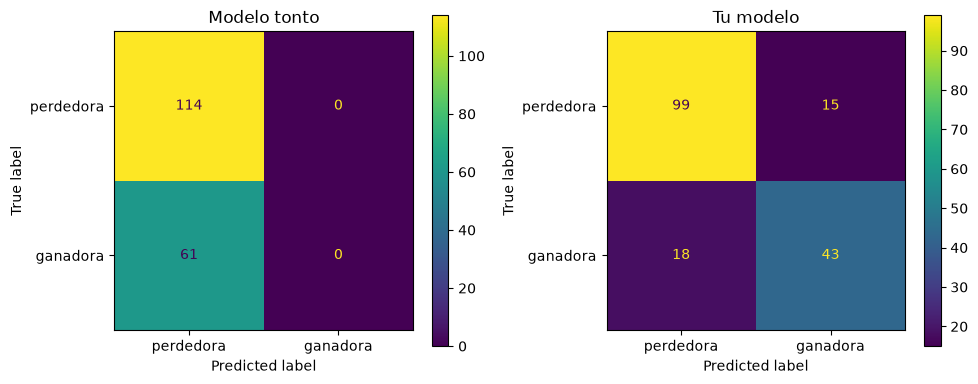
\includegraphics[keepaspectratio]{Copy_of_Laboratorio_4_files/73afac746650ef80dd6b9f6d7480827d618bb56e.png}}

\protect\phantomsection\label{RlA6GdrCnYyX}
\begin{quote}
\textbf{Responde aquí:} compara la exactitud y el F1 de los dos modelos.
¿Qué hace mal el modelo tonto que mirar únicamente la exactitud podría
ocultar?
\end{quote}

\textbf{Respuesta:} El modelo tonto solo predice la clase "false", no va
a poder ver la temporada ganadora porque jamás predice "True". Su
exactitud es solo el porcentaje de datos falsos, y su recall es cero.

\textbf{Exactitud:} el modelo tonto saca 0.651, el modelo real 0.811 ---
una mejora de 16 puntos. \textbf{F1:} el modelo tonto saca 0.000, el
modelo real 0.723 --- ahí la diferencia es total, no incremental.

Esa brecha en el F1 revela lo que la exactitud esconde: el modelo tonto
es tuerto, nunca predice \texttt{True} (siempre responde \texttt{False},
la clase más frecuente), así que su recall sobre
\texttt{ganadora\ =\ True} es 0 --- no detecta ni una sola temporada
ganadora. Aun así, como el 65 \% de las temporadas son \texttt{False},
acertar por pura repetición ya le da 0.651 de exactitud. Mirando solo la
exactitud, 0.651 no parece un desastre; el F1 en 0 deja claro que el
modelo tonto \textbf{ignora por completo la clase que nos interesa
detectar}.

\textbf{Recomendación} Será interesante probar con un modelo que
responda al azar en binomial con un porcentaje de aciertos determinado y
hacer varias corridas.

\protect\phantomsection\label{woA6HOc1nYyX}
\begin{center}\rule{0.5\linewidth}{0.5pt}\end{center}

\subsection{6 · Sacarlo de tu
computadora}\label{6--sacarlo-de-tu-computadora}

Hasta aquí solo había que ejecutar. \textbf{Esta parte sí la levantas
tú.}

Guardamos el \textbf{Pipeline completo} (escalador + modelo). Si
guardaras solo la regresión logística, la API recibiría datos sin
escalar y devolvería disparates \textbf{sin lanzar ningún error}.

\protect\phantomsection\label{uiPdQu81nYyY}
\begin{Shaded}
\begin{Highlighting}[]
\ImportTok{import}\NormalTok{ joblib, pathlib}

\NormalTok{pathlib.Path(}\StringTok{"modelos"}\NormalTok{).mkdir(exist\_ok}\OperatorTok{=}\VariableTok{True}\NormalTok{)}
\NormalTok{joblib.dump(modelo, }\StringTok{"modelos/modelo.joblib"}\NormalTok{)     }\CommentTok{\# el Pipeline ENTERO}
\BuiltInTok{print}\NormalTok{(}\StringTok{"modelos/modelo.joblib guardado"}\NormalTok{)}
\end{Highlighting}
\end{Shaded}

\begin{verbatim}
modelos/modelo.joblib guardado
\end{verbatim}

\protect\phantomsection\label{RpkclTf8nYyZ}
Estos dos archivos los necesita Docker:

\protect\phantomsection\label{41Bv3xLbnYyZ}
\begin{Shaded}
\begin{Highlighting}[]
\NormalTok{servir }\OperatorTok{=}\NormalTok{ [}
    \StringTok{"import joblib"}\NormalTok{,}
    \StringTok{"from fastapi import FastAPI"}\NormalTok{,}
    \StringTok{""}\NormalTok{,}
    \StringTok{\textquotesingle{}modelo = joblib.load("modelos/modelo.joblib")\textquotesingle{}}\NormalTok{,}
    \StringTok{\textquotesingle{}app = FastAPI(title="Temporada ganadora")\textquotesingle{}}\NormalTok{,}
    \StringTok{""}\NormalTok{,}
    \StringTok{\textquotesingle{}@app.get("/predecir")\textquotesingle{}}\NormalTok{,}
    \StringTok{"def predecir(gf: int, ga: int):"}\NormalTok{,}
    \StringTok{"    x = [[gf, ga, gf {-} ga]]"}\NormalTok{,}
    \StringTok{\textquotesingle{}    return \{"ganadora": bool(modelo.predict(x)[0]),\textquotesingle{}}\NormalTok{,}
    \StringTok{\textquotesingle{}            "probabilidad": round(float(modelo.predict\_proba(x)[0][1]), 3)\}\textquotesingle{}}\NormalTok{,}
\NormalTok{]}

\NormalTok{imagen }\OperatorTok{=}\NormalTok{ [}
    \StringTok{"FROM python:3.12{-}slim"}\NormalTok{,}
    \StringTok{"WORKDIR /app"}\NormalTok{,}
    \StringTok{"RUN pip install {-}{-}no{-}cache{-}dir fastapi uvicorn scikit{-}learn joblib"}\NormalTok{,}
    \StringTok{"COPY servir.py ."}\NormalTok{,}
    \StringTok{\textquotesingle{}CMD ["uvicorn", "servir:app", "{-}{-}host", "0.0.0.0", "{-}{-}port", "8000"]\textquotesingle{}}\NormalTok{,}
\NormalTok{]}

\BuiltInTok{open}\NormalTok{(}\StringTok{"servir.py"}\NormalTok{, }\StringTok{"w"}\NormalTok{, encoding}\OperatorTok{=}\StringTok{"utf{-}8"}\NormalTok{).write(}\StringTok{"}\CharTok{\textbackslash{}n}\StringTok{"}\NormalTok{.join(servir))}
\BuiltInTok{open}\NormalTok{(}\StringTok{"Dockerfile"}\NormalTok{, }\StringTok{"w"}\NormalTok{, encoding}\OperatorTok{=}\StringTok{"utf{-}8"}\NormalTok{).write(}\StringTok{"}\CharTok{\textbackslash{}n}\StringTok{"}\NormalTok{.join(imagen))}
\BuiltInTok{print}\NormalTok{(}\StringTok{"servir.py y Dockerfile escritos"}\NormalTok{)}
\end{Highlighting}
\end{Shaded}

\begin{verbatim}
servir.py y Dockerfile escritos
\end{verbatim}

\protect\phantomsection\label{bKJlMefZnYya}
En la \textbf{terminal}, dentro de esta carpeta:

\begin{Shaded}
\begin{Highlighting}[]
\ExtensionTok{docker}\NormalTok{ build }\AttributeTok{{-}t}\NormalTok{ nhl{-}api .}
\ExtensionTok{docker}\NormalTok{ run }\AttributeTok{{-}p}\NormalTok{ 8000:8000 }\AttributeTok{{-}v} \StringTok{"}\VariableTok{$\{PWD\}}\StringTok{/modelos:/app/modelos"}\NormalTok{ nhl{-}api}
\end{Highlighting}
\end{Shaded}

Abre \textbf{\url{http://localhost:8000/docs}}, prueba
\texttt{/predecir} con \texttt{gf=300} y \texttt{ga=250}, y captura la
respuesta.

\begin{itemize}
\tightlist
\item
  \texttt{-p\ 8000:8000} conecta el puerto del contenedor con el de tu
  máquina
\item
  \texttt{-v\ ...} mete tu carpeta \texttt{modelos/} dentro del
  contenedor
\end{itemize}

\begin{quote}
\textbf{Prueba esto:} corre el contenedor \textbf{sin} el \texttt{-v}.
¿Qué pasa y por qué?
\end{quote}

\protect\phantomsection\label{p99-bvZLnYyb}
\begin{center}\rule{0.5\linewidth}{0.5pt}\end{center}

\subsection{Entrega}\label{entrega}

En una celda de texto al final del notebook:

\begin{enumerate}
\tightlist
\item
  La exactitud y el F1 del \textbf{modelo tonto} y de \textbf{tu
  modelo}.
\item
  Qué hace mal el modelo tonto que la exactitud no deja ver.
\item
  Por qué se guarda el \textbf{Pipeline completo}
  (\texttt{StandardScaler} + \texttt{LogisticRegression}) y no solo la
  regresión logística.
\item
  Qué pasó al correr el contenedor \textbf{sin} \texttt{-v}.
\end{enumerate}

Y la \textbf{captura de la API respondiendo} en
\texttt{http://localhost:8000/docs}.

\begin{center}\rule{0.5\linewidth}{0.5pt}\end{center}

\begin{quote}
\textbf{Si haces la parte 7 (opcional)}, añade además:

\begin{itemize}
\tightlist
\item
  la \textbf{URL pública} de tu API
\item
  una captura de
  \texttt{https://\textless{}tu-dominio\textgreater{}/docs} con una
  llamada a \texttt{/predecir} que haya respondido bien
\end{itemize}
\end{quote}

\protect\phantomsection\label{amf75WIXnYyc}
\begin{center}\rule{0.5\linewidth}{0.5pt}\end{center}

\section{7 · Del localhost a Internet ·
OPCIONAL}\label{7--del-localhost-a-internet--opcional}

\begin{quote}
\textbf{Esta parte no es obligatoria.} El laboratorio ya está completo
con la entrega de arriba. Lo que sigue es para quien quiera dar el
último paso: que la API deje de vivir en tu computadora y quede
publicada en Internet, con una dirección que pueda abrir cualquiera.

Necesitas una cuenta de GitHub y unos 25 minutos.
\end{quote}

Tu API funciona\ldots{} \textbf{solo en tu computadora}. Eso es lo que
significa \texttt{localhost}: «esta misma máquina». Si cierras la
laptop, se acabó; y nadie más puede abrirla.

\begin{verbatim}
ANTES

Navegador (el tuyo)
     ↓
localhost:8000
     ↓
Contenedor Docker
     ↓
FastAPI
     ↓
modelo.joblib
\end{verbatim}

\begin{verbatim}
AHORA

Navegador de cualquier persona
          ↓
       Internet
          ↓
  servidor en la nube
          ↓
   Contenedor Docker
          ↓
       FastAPI
          ↓
    modelo.joblib
\end{verbatim}

Vamos a subir \textbf{el mismo contenedor} a un servidor en la nube y
obtener una URL pública. Usaremos \textbf{Railway}, porque construye la
aplicación a partir del \texttt{Dockerfile} que ya tienes: no hay que
aprender nada nuevo.

\begin{verbatim}
Proyecto local  →  GitHub  →  Railway  →  Dockerfile  →  contenedor  →  URL pública
\end{verbatim}

\protect\phantomsection\label{ZD6k47WHnYyd}
\subsubsection{Primero: que el modelo viaje dentro de la
imagen}\label{primero-que-el-modelo-viaje-dentro-de-la-imagen}

En local, el modelo entraba al contenedor \textbf{desde tu carpeta}, con
\texttt{-v}:

\begin{verbatim}
TU COMPUTADORA              CONTENEDOR
modelos/                    /app/modelos/
└── modelo.joblib    -v →   └── modelo.joblib
\end{verbatim}

Pero en la nube \textbf{no existe tu carpeta}. El servidor no tiene un
\texttt{modelos/} que montar. Así que cambiamos la estrategia: metemos
el modelo \textbf{dentro de la imagen} al construirla.

\begin{verbatim}
modelo.joblib  →  docker build  →  queda dentro de la imagen
\end{verbatim}

Eso no significa que el \texttt{-v} estuviera mal. Son \textbf{dos
formas distintas} de hacer que un archivo esté disponible dentro de un
contenedor: montarlo desde fuera, o copiarlo adentro.

\protect\phantomsection\label{hlBHzqACnYyd}
\begin{Shaded}
\begin{Highlighting}[]
\NormalTok{imagen\_nube }\OperatorTok{=}\NormalTok{ [}
    \StringTok{"FROM python:3.12{-}slim"}\NormalTok{,}
    \StringTok{"WORKDIR /app"}\NormalTok{,}
    \StringTok{"RUN pip install {-}{-}no{-}cache{-}dir fastapi uvicorn scikit{-}learn joblib"}\NormalTok{,}
    \StringTok{"COPY servir.py ."}\NormalTok{,}
    \StringTok{"COPY modelos ./modelos"}\NormalTok{,                      }\CommentTok{\# ← el modelo entra a la imagen}
    \StringTok{\textquotesingle{}CMD ["sh", "{-}c", "uvicorn servir:app {-}{-}host 0.0.0.0 {-}{-}port $}\SpecialCharTok{\{PORT:{-}8000\}}\StringTok{"]\textquotesingle{}}\NormalTok{,}
\NormalTok{]}

\BuiltInTok{open}\NormalTok{(}\StringTok{"Dockerfile"}\NormalTok{, }\StringTok{"w"}\NormalTok{, encoding}\OperatorTok{=}\StringTok{"utf{-}8"}\NormalTok{).write(}\StringTok{"}\CharTok{\textbackslash{}n}\StringTok{"}\NormalTok{.join(imagen\_nube))}
\BuiltInTok{print}\NormalTok{(}\StringTok{"Dockerfile actualizado para la nube"}\NormalTok{)}
\BuiltInTok{print}\NormalTok{()}
\BuiltInTok{print}\NormalTok{(}\BuiltInTok{open}\NormalTok{(}\StringTok{"Dockerfile"}\NormalTok{, encoding}\OperatorTok{=}\StringTok{"utf{-}8"}\NormalTok{).read())}
\end{Highlighting}
\end{Shaded}

\begin{verbatim}
Dockerfile actualizado para la nube

FROM python:3.12-slim
WORKDIR /app
RUN pip install --no-cache-dir fastapi uvicorn scikit-learn joblib
COPY servir.py .
COPY modelos ./modelos
CMD ["sh", "-c", "uvicorn servir:app --host 0.0.0.0 --port ${PORT:-8000}"]
\end{verbatim}

\protect\phantomsection\label{txM86Nk6nYye}
Dos líneas nuevas:

\textbf{\texttt{COPY\ modelos\ ./modelos}} --- copia tu carpeta
\texttt{modelos/} (con el \texttt{.joblib} dentro) a la imagen. Ya no
hace falta \texttt{-v}.

\textbf{\texttt{-\/-port\ \$\{PORT:-8000\}}} --- así se lee:

\begin{verbatim}
¿existe una variable PORT?
   sí  →  usa ese puerto
   no  →  usa 8000
\end{verbatim}

En tu computadora \texttt{PORT} no está definido, así que sigue siendo
el 8000 de siempre. En la nube, \textbf{la plataforma decide el puerto}
y te lo pasa en esa variable. Con esto el mismo Dockerfile sirve en los
dos sitios.

\protect\phantomsection\label{Y0lyk4Q9nYyf}
\subsubsection{Subir el proyecto a
GitHub}\label{subir-el-proyecto-a-github}

Railway lee tu código desde GitHub. En el repositorio tienen que estar,
como mínimo, estos tres:

\begin{verbatim}
Dockerfile
servir.py
modelos/modelo.joblib
\end{verbatim}

Desde la terminal, en la carpeta del proyecto:

\begin{Shaded}
\begin{Highlighting}[]
\FunctionTok{git}\NormalTok{ add .}
\FunctionTok{git}\NormalTok{ commit }\AttributeTok{{-}m} \StringTok{"Deploy NHL API"}
\FunctionTok{git}\NormalTok{ push}
\end{Highlighting}
\end{Shaded}

Si aún no tienes repositorio, créalo en GitHub y sigue las instrucciones
que la propia página te muestra al crearlo.

\begin{quote}
\textbf{Ojo:} si tienes un \texttt{.gitignore} que ignora
\texttt{*.joblib} o la carpeta \texttt{modelos/}, el modelo \textbf{no
se sube} y el despliegue falla. Comprueba con \texttt{git\ status} que
el \texttt{.joblib} aparece entre los archivos añadidos.
\end{quote}

\protect\phantomsection\label{6fh9nPP1nYyf}
\subsubsection{Desplegar en Railway}\label{desplegar-en-railway}

El flujo, sin depender de cómo se llamen los botones hoy:

\begin{enumerate}
\tightlist
\item
  Entra a \textbf{Railway} y crea una cuenta (puedes usar la de GitHub).
\item
  Crea un \textbf{proyecto nuevo}.
\item
  Elige desplegar \textbf{desde un repositorio de GitHub}.
\item
  Selecciona el repositorio de este laboratorio.
\item
  Railway detecta el \texttt{Dockerfile} y \textbf{construye la imagen}.
  Tarda unos minutos: está haciendo lo mismo que hizo tu
  \texttt{docker\ build}, pero en su servidor.
\item
  Cuando termina, \textbf{arranca el contenedor}.
\item
  En la configuración del servicio, \textbf{genera un dominio público}.
\item
  Abre esa URL.
\end{enumerate}

Tu dirección será algo parecido a esto (\textbf{es solo un ejemplo, no
la copies}):

\begin{verbatim}
https://mi-nhl-api.up.railway.app/docs
\end{verbatim}

Ahí tienes la misma página \texttt{/docs} que viste en
\texttt{localhost}, pero servida desde Internet. Prueba
\texttt{GET\ /predecir} con \texttt{gf\ =\ 300} y \texttt{ga\ =\ 250}.
Debería responder algo con esta forma:

\begin{Shaded}
\begin{Highlighting}[]
\FunctionTok{\{}
  \DataTypeTok{"ganadora"}\FunctionTok{:} \KeywordTok{true}\FunctionTok{,}
  \DataTypeTok{"probabilidad"}\FunctionTok{:} \FloatTok{0.87}
\FunctionTok{\}}
\end{Highlighting}
\end{Shaded}

El número exacto depende de tu modelo; lo que importa es que responda.

\protect\phantomsection\label{3614f0f4}
\section{Actividad --- De la web a una
API}\label{actividad--de-la-web-a-una-api}

Bajas estadísticas de equipos de la NHL, entrenas un modelo que predice
si una temporada fue ganadora, y lo dejas respondiendo dentro de un
contenedor.

Al final hay una parte \textbf{opcional}: publicarlo en Internet con una
URL que pueda abrir cualquiera.

\textbf{El código de Python ya está escrito.} Tu trabajo es ejecutarlo,
entender qué pasa en cada paso y responder las preguntas. Lo que sí
tienes que hacer funcionar por tu cuenta es la \textbf{API} y el
\textbf{contenedor}.

\textbf{Entregas:} este notebook ejecutado + una captura de la API
respondiendo.

\protect\phantomsection\label{685c3e12}
\begin{center}\rule{0.5\linewidth}{0.5pt}\end{center}

\subsection{Antes de empezar: ¿qué vamos a
predecir?}\label{antes-de-empezar-quuxe9-vamos-a-predecir}

Cada fila de los datos son \textbf{las estadísticas de un equipo de la
NHL en una temporada}. El scraper construye estas nueve columnas:

\begin{Shaded}
\begin{Highlighting}[]
\NormalTok{COLS }\OperatorTok{=}\NormalTok{ [}\StringTok{"equipo"}\NormalTok{, }\StringTok{"anio"}\NormalTok{, }\StringTok{"victorias"}\NormalTok{, }\StringTok{"derrotas"}\NormalTok{, }\StringTok{"ot"}\NormalTok{,}
        \StringTok{"win\_pct"}\NormalTok{, }\StringTok{"gf"}\NormalTok{, }\StringTok{"ga"}\NormalTok{, }\StringTok{"dif"}\NormalTok{]}
\end{Highlighting}
\end{Shaded}

Las cuatro que importan hoy:

{\def\LTcaptype{none} % do not increment counter
\begin{longtable}[]{@{}ll@{}}
\toprule\noalign{}
columna & qué es \\
\midrule\noalign{}
\endhead
\bottomrule\noalign{}
\endlastfoot
\texttt{gf} & \emph{goals for} --- goles que \textbf{anotó} el equipo \\
\texttt{ga} & \emph{goals against} --- goles que \textbf{recibió} \\
\texttt{dif} & la diferencia: \texttt{gf\ -\ ga} \\
\texttt{win\_pct} & la proporción de partidos ganados \\
\end{longtable}
}

Así se ve, en concreto:

\begin{verbatim}
equipo     gf    ga    dif    win_pct
Boston     300   220     80      0.67
Detroit    210   280    -70      0.38
\end{verbatim}

Boston anotó 80 goles más de los que recibió y ganó el 67 \% de sus
partidos. Detroit recibió 70 más de los que anotó y ganó el 38 \%.

\textbf{La pregunta que va a responder el modelo:}

\begin{quote}
Sabiendo cuántos goles anotó un equipo y cuántos recibió, ¿su temporada
fue \textbf{ganadora}?
\end{quote}

Un detalle importante: la respuesta (\emph{ganadora} sí o no) \textbf{no
viene en la tabla}. La vamos a construir nosotros en la parte 2.

\protect\phantomsection\label{6ea3c1a2}
\begin{center}\rule{0.5\linewidth}{0.5pt}\end{center}

\subsection{0 · Las librerías}\label{0--las-libreruxedas}

Ejecuta esta celda una vez. \texttt{pyarrow} es el motor que necesita
Pandas para escribir archivos \textbf{Parquet}; sin él, el
\texttt{to\_parquet} de la parte 1 falla.

\protect\phantomsection\label{e40e74a9}
\begin{Shaded}
\begin{Highlighting}[]
\CommentTok{\# se ejecuta una sola vez; si ya están instaladas, no hace nada}
\OperatorTok{\%}\NormalTok{pip install }\OperatorTok{{-}}\NormalTok{q requests beautifulsoup4 pandas pyarrow scikit}\OperatorTok{{-}}\NormalTok{learn joblib matplotlib}
\end{Highlighting}
\end{Shaded}

\begin{verbatim}
Note: you may need to restart the kernel to use updated packages.
\end{verbatim}

\protect\phantomsection\label{494fabd0}
\begin{center}\rule{0.5\linewidth}{0.5pt}\end{center}

\subsection{1 · Bajar los datos}\label{1--bajar-los-datos}

La página muestra 100 equipos por vez y se pagina con
\texttt{?page\_num=}. Primero probamos \textbf{una} página.

\protect\phantomsection\label{17fefd72}
\begin{Shaded}
\begin{Highlighting}[]
\ImportTok{import}\NormalTok{ time}
\ImportTok{import}\NormalTok{ requests}
\ImportTok{import}\NormalTok{ pandas }\ImportTok{as}\NormalTok{ pd}
\ImportTok{from}\NormalTok{ bs4 }\ImportTok{import}\NormalTok{ BeautifulSoup}

\NormalTok{URL }\OperatorTok{=} \StringTok{"https://www.scrapethissite.com/pages/forms/?page\_num=}\SpecialCharTok{\{\}}\StringTok{\&per\_page=100"}
\NormalTok{COLS }\OperatorTok{=}\NormalTok{ [}\StringTok{"equipo"}\NormalTok{, }\StringTok{"anio"}\NormalTok{, }\StringTok{"victorias"}\NormalTok{, }\StringTok{"derrotas"}\NormalTok{, }\StringTok{"ot"}\NormalTok{, }\StringTok{"win\_pct"}\NormalTok{,}
        \StringTok{"gf"}\NormalTok{, }\StringTok{"ga"}\NormalTok{, }\StringTok{"dif"}\NormalTok{]}

\KeywordTok{def}\NormalTok{ leer\_pagina(n):}
    \CommentTok{"""Devuelve las filas de una página como lista de diccionarios."""}
\NormalTok{    sopa }\OperatorTok{=}\NormalTok{ BeautifulSoup(requests.get(URL.}\BuiltInTok{format}\NormalTok{(n), timeout}\OperatorTok{=}\DecValTok{20}\NormalTok{).text,}
                         \StringTok{"html.parser"}\NormalTok{)}
\NormalTok{    filas }\OperatorTok{=}\NormalTok{ []}
    \ControlFlowTok{for}\NormalTok{ tr }\KeywordTok{in}\NormalTok{ sopa.select(}\StringTok{"tr.team"}\NormalTok{):                 }\CommentTok{\# ← el selector CSS}
\NormalTok{        celdas }\OperatorTok{=}\NormalTok{ [td.text.strip() }\ControlFlowTok{for}\NormalTok{ td }\KeywordTok{in}\NormalTok{ tr.select(}\StringTok{"td"}\NormalTok{)]}
\NormalTok{        filas.append(}\BuiltInTok{dict}\NormalTok{(}\BuiltInTok{zip}\NormalTok{(COLS, celdas)))}
    \ControlFlowTok{return}\NormalTok{ filas}

\BuiltInTok{print}\NormalTok{(}\BuiltInTok{len}\NormalTok{(leer\_pagina(}\DecValTok{1}\NormalTok{)), }\StringTok{"filas en la página 1"}\NormalTok{)}
\end{Highlighting}
\end{Shaded}

\begin{verbatim}
100 filas en la página 1
\end{verbatim}

\protect\phantomsection\label{ac26ed8f}
Ahora las seis.

\begin{quote}
\textbf{Si la página no responde} (se cayó el sitio, la red la bloquea,
cambió el HTML): no pierdas la mañana. En el aula virtual está
\textbf{\texttt{equipos\_respaldo.csv}} con las mismas 582 filas. Súbelo
a esta carpeta y usa esta línea en lugar de la celda de abajo:

\begin{Shaded}
\begin{Highlighting}[]
\NormalTok{equipos }\OperatorTok{=}\NormalTok{ pd.read\_csv(}\StringTok{"equipos\_respaldo.csv"}\NormalTok{)}
\end{Highlighting}
\end{Shaded}

Todo lo que sigue funciona igual.
\end{quote}

\protect\phantomsection\label{2c8affdc}
\begin{Shaded}
\begin{Highlighting}[]
\NormalTok{datos }\OperatorTok{=}\NormalTok{ []}

\ControlFlowTok{for}\NormalTok{ n }\KeywordTok{in} \BuiltInTok{range}\NormalTok{(}\DecValTok{1}\NormalTok{, }\DecValTok{7}\NormalTok{):            }\CommentTok{\# 6 páginas × 100 filas}
\NormalTok{    datos }\OperatorTok{+=}\NormalTok{ leer\_pagina(n)}
    \BuiltInTok{print}\NormalTok{(}\SpecialStringTok{f"página }\SpecialCharTok{\{}\NormalTok{n}\SpecialCharTok{\}}\SpecialStringTok{"}\NormalTok{, end}\OperatorTok{=}\StringTok{"  "}\NormalTok{)}
\NormalTok{    time.sleep(}\FloatTok{0.5}\NormalTok{)              }\CommentTok{\# educación: una pausa entre pedidos}

\BuiltInTok{print}\NormalTok{(}\StringTok{"}\CharTok{\textbackslash{}n}\StringTok{"}\NormalTok{, }\BuiltInTok{len}\NormalTok{(datos), }\StringTok{"filas"}\NormalTok{)}
\end{Highlighting}
\end{Shaded}

\begin{verbatim}
página 1  página 2  página 3  página 4  página 5  página 6  
 582 filas
\end{verbatim}

\protect\phantomsection\label{3fa2baa4}
Lo que llega de la web es \textbf{texto}: \texttt{"44"} no es el número
44. Hay que convertirlo antes de poder calcular nada.

Guardamos el resultado en los dos formatos que vimos esta semana, para
compararlos.

\protect\phantomsection\label{24d3c94b}
\begin{Shaded}
\begin{Highlighting}[]
\NormalTok{equipos }\OperatorTok{=}\NormalTok{ pd.DataFrame(datos)}

\CommentTok{\# lo que llega de la web es TEXTO: hay que convertirlo a número}
\ControlFlowTok{for}\NormalTok{ c }\KeywordTok{in}\NormalTok{ [}\StringTok{"anio"}\NormalTok{, }\StringTok{"victorias"}\NormalTok{, }\StringTok{"derrotas"}\NormalTok{, }\StringTok{"gf"}\NormalTok{, }\StringTok{"ga"}\NormalTok{, }\StringTok{"dif"}\NormalTok{]:}
\NormalTok{    equipos[c] }\OperatorTok{=}\NormalTok{ pd.to\_numeric(equipos[c], errors}\OperatorTok{=}\StringTok{"coerce"}\NormalTok{)}
\NormalTok{equipos[}\StringTok{"win\_pct"}\NormalTok{] }\OperatorTok{=}\NormalTok{ pd.to\_numeric(equipos[}\StringTok{"win\_pct"}\NormalTok{], errors}\OperatorTok{=}\StringTok{"coerce"}\NormalTok{)}

\NormalTok{equipos.to\_csv(}\StringTok{"equipos.csv"}\NormalTok{, index}\OperatorTok{=}\VariableTok{False}\NormalTok{)}
\NormalTok{equipos.to\_parquet(}\StringTok{"equipos.parquet"}\NormalTok{, index}\OperatorTok{=}\VariableTok{False}\NormalTok{)   }\CommentTok{\# necesita pyarrow}

\ImportTok{import}\NormalTok{ os}
\BuiltInTok{print}\NormalTok{(}\SpecialStringTok{f"csv     }\SpecialCharTok{\{}\NormalTok{os}\SpecialCharTok{.}\NormalTok{path}\SpecialCharTok{.}\NormalTok{getsize(}\StringTok{\textquotesingle{}equipos.csv\textquotesingle{}}\NormalTok{)}\OperatorTok{/}\DecValTok{1024}\SpecialCharTok{:6.1f\}}\SpecialStringTok{ KB"}\NormalTok{)}
\BuiltInTok{print}\NormalTok{(}\SpecialStringTok{f"parquet }\SpecialCharTok{\{}\NormalTok{os}\SpecialCharTok{.}\NormalTok{path}\SpecialCharTok{.}\NormalTok{getsize(}\StringTok{\textquotesingle{}equipos.parquet\textquotesingle{}}\NormalTok{)}\OperatorTok{/}\DecValTok{1024}\SpecialCharTok{:6.1f\}}\SpecialStringTok{ KB"}\NormalTok{)}
\NormalTok{equipos.head(}\DecValTok{3}\NormalTok{)}
\end{Highlighting}
\end{Shaded}

\begin{verbatim}
csv       27.1 KB
parquet   12.7 KB
\end{verbatim}

\begin{verbatim}
           equipo  anio  victorias  derrotas ot  win_pct   gf   ga  dif
0   Boston Bruins  1990         44        24       0.550  299  264   35
1  Buffalo Sabres  1990         31        30       0.388  292  278   14
2  Calgary Flames  1990         46        26       0.575  344  263   81
\end{verbatim}

\protect\phantomsection\label{cc48ef23}
\begin{quote}
\textbf{Anota} los dos tamaños. ¿Te sorprende cuál gana?
\end{quote}

\textbf{Respuesta:}: Los equipos canadienses son mas naturales para
jugar hockey que en los EE.UU.

\protect\phantomsection\label{f860ece2}
\begin{center}\rule{0.5\linewidth}{0.5pt}\end{center}

\subsection{2 · La variable objetivo}\label{2--la-variable-objetivo}

Los datos no traen una columna que diga «esta temporada fue buena». La
creamos nosotros a partir de \texttt{win\_pct}, con una regla sencilla:

\[
\text{ganadora} =
\begin{cases}
\text{True}, & \text{si } win\_pct > 0.5 \\
\text{False}, & \text{si } win\_pct \le 0.5
\end{cases}
\]

En ejemplos:

\begin{verbatim}
win_pct = 0.65  ->  ganadora = True
win_pct = 0.54  ->  ganadora = True
win_pct = 0.50  ->  ganadora = False     ← ojo
win_pct = 0.42  ->  ganadora = False
\end{verbatim}

\textbf{Fíjate en el tercero.} Usamos \texttt{\textgreater{}\ 0.5}, no
\texttt{\textgreater{}=\ 0.5}. Una temporada con exactamente la mitad de
partidos ganados \textbf{no} cuenta como ganadora. Es una decisión
nuestra, y podría haber sido la contraria: así de concretas son las
definiciones en un problema real.

A esta columna se la llama \textbf{variable objetivo} (o \emph{target},
o \emph{etiqueta}): es lo que queremos que el modelo aprenda a predecir.

\protect\phantomsection\label{d6765b21}
\begin{Shaded}
\begin{Highlighting}[]
\NormalTok{equipos[}\StringTok{"ganadora"}\NormalTok{] }\OperatorTok{=}\NormalTok{ equipos[}\StringTok{"win\_pct"}\NormalTok{] }\OperatorTok{\textgreater{}} \FloatTok{0.5}

\NormalTok{equipos[[}\StringTok{"equipo"}\NormalTok{, }\StringTok{"anio"}\NormalTok{, }\StringTok{"gf"}\NormalTok{, }\StringTok{"ga"}\NormalTok{, }\StringTok{"dif"}\NormalTok{, }\StringTok{"win\_pct"}\NormalTok{, }\StringTok{"ganadora"}\NormalTok{]].head()}
\end{Highlighting}
\end{Shaded}

\begin{verbatim}
               equipo  anio   gf   ga  dif  win_pct  ganadora
0       Boston Bruins  1990  299  264   35    0.550      True
1      Buffalo Sabres  1990  292  278   14    0.388     False
2      Calgary Flames  1990  344  263   81    0.575      True
3  Chicago Blackhawks  1990  284  211   73    0.613      True
4   Detroit Red Wings  1990  273  298  -25    0.425     False
\end{verbatim}

\protect\phantomsection\label{e22f6750}
Ahora veamos \textbf{cuántas temporadas hay de cada tipo}.

\texttt{value\_counts(normalize=True)} cuenta cuántas filas hay de cada
valor y lo convierte en proporción. Si sale algo como:

\begin{verbatim}
False    0.71
True     0.29
\end{verbatim}

significa que el \textbf{71 \% de las temporadas no fueron ganadoras} y
el \textbf{29 \% sí}.

Dos aclaraciones que evitan confusiones:

\begin{itemize}
\tightlist
\item
  Esos números \textbf{no son predicciones de ningún modelo}. Todavía no
  hemos entrenado nada. Es simplemente cómo están repartidos los datos.
\item
  Como no están cerca de 50 \% y 50 \%, decimos que las clases están
  \textbf{desbalanceadas}. Recuerda ese detalle: va a ser importante en
  un rato.
\end{itemize}

La segunda tabla muestra la diferencia media de goles en cada grupo. Si
los dos números son muy distintos, es buena señal: significa que
\texttt{dif} \textbf{sí} distingue los dos tipos de temporada.

\protect\phantomsection\label{e722cc47}
\begin{Shaded}
\begin{Highlighting}[]
\BuiltInTok{print}\NormalTok{(equipos[}\StringTok{"ganadora"}\NormalTok{].value\_counts(normalize}\OperatorTok{=}\VariableTok{True}\NormalTok{).}\BuiltInTok{round}\NormalTok{(}\DecValTok{2}\NormalTok{))}
\BuiltInTok{print}\NormalTok{()}
\BuiltInTok{print}\NormalTok{(}\StringTok{"diferencia media de goles en cada grupo:"}\NormalTok{)}
\BuiltInTok{print}\NormalTok{(equipos.groupby(}\StringTok{"ganadora"}\NormalTok{)[}\StringTok{"dif"}\NormalTok{].mean().}\BuiltInTok{round}\NormalTok{(}\DecValTok{1}\NormalTok{))}
\end{Highlighting}
\end{Shaded}

\begin{verbatim}
ganadora
False    0.65
True     0.35
Name: proportion, dtype: float64

diferencia media de goles en cada grupo:
ganadora
False   -21.3
True     40.2
Name: dif, dtype: float64
\end{verbatim}

\protect\phantomsection\label{8c7d753c}
\begin{center}\rule{0.5\linewidth}{0.5pt}\end{center}

\subsection{\texorpdfstring{3 · \texttt{X} e \texttt{y}: lo que ve el
modelo y lo que debe
adivinar}{3 · X e y: lo que ve el modelo y lo que debe adivinar}}\label{3--x-e-y-lo-que-ve-el-modelo-y-lo-que-debe-adivinar}

Para entrenar cualquier modelo hay que separar los datos en dos cosas.

\subsubsection{\texorpdfstring{\texttt{X} --- las características
(\emph{features})}{X --- las características (features)}}\label{x--las-caracteruxedsticas-features}

Son las columnas que el modelo \textbf{puede mirar} para decidir:

\begin{verbatim}
X

gf    ga    dif
300   250    50
210   270   -60
280   260    20
\end{verbatim}

\begin{itemize}
\tightlist
\item
  cada \textbf{fila} es la temporada de un equipo
\item
  cada \textbf{columna} es una característica
\end{itemize}

Si hay \texttt{n} temporadas, \texttt{X} tiene forma \(n \times 3\):
\texttt{n} filas y 3 características.

\subsubsection{\texorpdfstring{\texttt{y} --- la variable objetivo
(\emph{target})}{y --- la variable objetivo (target)}}\label{y--la-variable-objetivo-target}

Es la respuesta correcta de cada fila:

\begin{verbatim}
y

True
False
True
\end{verbatim}

\subsubsection{Cómo se relacionan}\label{cuxf3mo-se-relacionan}

Cada fila de \texttt{X} tiene su respuesta en \texttt{y}, en la misma
posición:

\begin{verbatim}
gf    ga    dif        ganadora
300   250    50   ->     True
210   270   -60   ->     False
280   260    20   ->     True
\end{verbatim}

Eso es el \textbf{aprendizaje supervisado}: darle al modelo muchos pares
\emph{(pregunta, respuesta)} para que encuentre la relación

\[X \longrightarrow y\]

o dicho en palabras:

\begin{verbatim}
[goles a favor, goles en contra, diferencia]
                    ↓
              ¿ganadora o no?
\end{verbatim}

\protect\phantomsection\label{e1501fd2}
\begin{Shaded}
\begin{Highlighting}[]
\NormalTok{X }\OperatorTok{=}\NormalTok{ equipos[[}\StringTok{"gf"}\NormalTok{, }\StringTok{"ga"}\NormalTok{, }\StringTok{"dif"}\NormalTok{]]    }\CommentTok{\# lo que el modelo VE}
\NormalTok{y }\OperatorTok{=}\NormalTok{ equipos[}\StringTok{"ganadora"}\NormalTok{]             }\CommentTok{\# lo que el modelo debe ADIVINAR}

\BuiltInTok{print}\NormalTok{(}\StringTok{"X:"}\NormalTok{, X.shape, }\StringTok{" {-}\textgreater{} (filas, características)"}\NormalTok{)}
\BuiltInTok{print}\NormalTok{(}\StringTok{"y:"}\NormalTok{, y.shape)}
\NormalTok{X.head(}\DecValTok{3}\NormalTok{)}
\end{Highlighting}
\end{Shaded}

\begin{verbatim}
X: (582, 3)  -> (filas, características)
y: (582,)
\end{verbatim}

\begin{verbatim}
    gf   ga  dif
0  299  264   35
1  292  278   14
2  344  263   81
\end{verbatim}

\protect\phantomsection\label{5f27ae0f}
Y ahora partimos los datos en dos:

\begin{itemize}
\tightlist
\item
  \textbf{entrenamiento (70 \%)} --- el modelo los estudia
\item
  \textbf{prueba (30 \%)} --- el modelo \textbf{nunca} los ve durante el
  entrenamiento; sirven para medir si de verdad aprendió o solo memorizó
\end{itemize}

\texttt{stratify=y} mantiene la misma proporción de ganadoras en los dos
grupos. Sin eso, por azar, el grupo de prueba podría quedar con muy
pocas.

\protect\phantomsection\label{679f4a20}
\begin{Shaded}
\begin{Highlighting}[]
\ImportTok{from}\NormalTok{ sklearn.model\_selection }\ImportTok{import}\NormalTok{ train\_test\_split}

\NormalTok{X\_tr, X\_te, y\_tr, y\_te }\OperatorTok{=}\NormalTok{ train\_test\_split(}
\NormalTok{    X, y, test\_size}\OperatorTok{=}\FloatTok{0.3}\NormalTok{, stratify}\OperatorTok{=}\NormalTok{y, random\_state}\OperatorTok{=}\DecValTok{0}\NormalTok{)}

\BuiltInTok{print}\NormalTok{(}\SpecialStringTok{f"entrenamiento: }\SpecialCharTok{\{}\BuiltInTok{len}\NormalTok{(X\_tr)}\SpecialCharTok{\}}\SpecialStringTok{ filas"}\NormalTok{)}
\BuiltInTok{print}\NormalTok{(}\SpecialStringTok{f"prueba:        }\SpecialCharTok{\{}\BuiltInTok{len}\NormalTok{(X\_te)}\SpecialCharTok{\}}\SpecialStringTok{ filas"}\NormalTok{)}
\end{Highlighting}
\end{Shaded}

\begin{verbatim}
entrenamiento: 407 filas
prueba:        175 filas
\end{verbatim}

\protect\phantomsection\label{e256d7e9}
\begin{center}\rule{0.5\linewidth}{0.5pt}\end{center}

\subsection{4 · Primero, el modelo
tonto}\label{4--primero-el-modelo-tonto}

Antes de entrenar nada serio, necesitamos saber \textbf{contra qué
comparar}. A ese punto de referencia se le llama \textbf{baseline}.

\texttt{DummyClassifier(strategy="most\_frequent")} hace lo más simple
imaginable: mira cuál es la clase más frecuente en el entrenamiento y
\textbf{responde siempre esa}, sin mirar \texttt{gf}, \texttt{ga} ni
\texttt{dif}.

Si la mayoría de las temporadas son perdedoras, el modelo tonto
responde:

\begin{verbatim}
False
False
False
False
...
\end{verbatim}

Y acierta bastante, solo por repetir la respuesta más común:

\begin{verbatim}
Real       Predicción del tonto
False      False   ✓
False      False   ✓
True       False   ✗
False      False   ✓
True       False   ✗
\end{verbatim}

\textbf{Para qué sirve esto.} Antes de decir «mi modelo tiene 90 \% de
exactitud», hay que responder: \emph{¿es mejor que esta estrategia que
ni siquiera mira los datos?} Si tu modelo saca 0.67 y el tonto saca
0.65, no has construido nada.

\begin{quote}
Un modelo útil tiene que ganarle al baseline \textbf{por un margen
claro}.
\end{quote}

\protect\phantomsection\label{94bd3b4c}
\begin{Shaded}
\begin{Highlighting}[]
\ImportTok{from}\NormalTok{ sklearn.dummy }\ImportTok{import}\NormalTok{ DummyClassifier}
\ImportTok{from}\NormalTok{ sklearn.metrics }\ImportTok{import}\NormalTok{ accuracy\_score, f1\_score}

\NormalTok{tonto }\OperatorTok{=}\NormalTok{ DummyClassifier(strategy}\OperatorTok{=}\StringTok{"most\_frequent"}\NormalTok{).fit(X\_tr, y\_tr)}
\NormalTok{p }\OperatorTok{=}\NormalTok{ tonto.predict(X\_te)}

\BuiltInTok{print}\NormalTok{(}\StringTok{"sus 5 primeras predicciones:"}\NormalTok{, p[:}\DecValTok{5}\NormalTok{])}
\BuiltInTok{print}\NormalTok{(}\SpecialStringTok{f"MODELO TONTO   exactitud }\SpecialCharTok{\{}\NormalTok{accuracy\_score(y\_te, p)}\SpecialCharTok{:.3f\}}\SpecialStringTok{"}
      \SpecialStringTok{f"   F1 }\SpecialCharTok{\{}\NormalTok{f1\_score(y\_te, p)}\SpecialCharTok{:.3f\}}\SpecialStringTok{"}\NormalTok{)}
\end{Highlighting}
\end{Shaded}

\begin{verbatim}
sus 5 primeras predicciones: [False False False False False]
MODELO TONTO   exactitud 0.651   F1 0.000
\end{verbatim}

\protect\phantomsection\label{3e6dfdc9}
\begin{quote}
\textbf{Anota ese número.} Es el que tu modelo tiene que superar.
\end{quote}

\protect\phantomsection\label{4cae6374}
\begin{center}\rule{0.5\linewidth}{0.5pt}\end{center}

\subsection{5 · Entrenar el modelo de
verdad}\label{5--entrenar-el-modelo-de-verdad}

Usamos un \textbf{Pipeline} con dos pasos:

\begin{enumerate}
\tightlist
\item
  \texttt{StandardScaler} --- pone las tres columnas en la misma escala
\item
  \texttt{LogisticRegression} --- el clasificador
\end{enumerate}

Guardarlos juntos importa: cuando el modelo salga a producir
predicciones, los datos nuevos tendrán que pasar por
\textbf{exactamente} las mismas transformaciones.

\protect\phantomsection\label{a850a8aa}
\begin{Shaded}
\begin{Highlighting}[]
\ImportTok{from}\NormalTok{ sklearn.pipeline }\ImportTok{import}\NormalTok{ make\_pipeline}
\ImportTok{from}\NormalTok{ sklearn.preprocessing }\ImportTok{import}\NormalTok{ StandardScaler}
\ImportTok{from}\NormalTok{ sklearn.linear\_model }\ImportTok{import}\NormalTok{ LogisticRegression}

\NormalTok{modelo }\OperatorTok{=}\NormalTok{ make\_pipeline(StandardScaler(), LogisticRegression(max\_iter}\OperatorTok{=}\DecValTok{5000}\NormalTok{))}
\NormalTok{modelo.fit(X\_tr, y\_tr)}

\NormalTok{pred }\OperatorTok{=}\NormalTok{ modelo.predict(X\_te)}
\BuiltInTok{print}\NormalTok{(}\SpecialStringTok{f"TU MODELO      exactitud }\SpecialCharTok{\{}\NormalTok{accuracy\_score(y\_te, pred)}\SpecialCharTok{:.3f\}}\SpecialStringTok{"}
      \SpecialStringTok{f"   F1 }\SpecialCharTok{\{}\NormalTok{f1\_score(y\_te, pred)}\SpecialCharTok{:.3f\}}\SpecialStringTok{"}\NormalTok{)}
\end{Highlighting}
\end{Shaded}

\begin{verbatim}
TU MODELO      exactitud 0.811   F1 0.723
\end{verbatim}

\protect\phantomsection\label{740f66c3}
Compara los resultados con los del modelo tonto. Mira \textbf{tanto la
exactitud como el F1}, porque las dos métricas no cuentan exactamente la
misma historia.

\subsubsection{Qué miden precision, recall y
F1}\label{quuxe9-miden-precision-recall-y-f1}

Nos centramos en la clase que nos interesa detectar:
\texttt{ganadora\ =\ True}.

\textbf{Precisión} --- de todas las que el modelo \emph{dijo} que eran
ganadoras, ¿cuántas lo eran de verdad?

\[Precision = \frac{TP}{TP + FP}\]

\textbf{Recall} --- de todas las que \emph{realmente} eran ganadoras,
¿cuántas encontró?

\[Recall = \frac{TP}{TP + FN}\]

\textbf{F1} --- combina las dos en un solo número:

\[F1 = 2 \cdot \frac{Precision \cdot Recall}{Precision + Recall}\]

Lo único que hay que recordar de esa fórmula: \textbf{el F1 solo es alto
si las dos son altas}. Si una de las dos se hunde, el F1 se hunde con
ella.

\subsubsection{Por qué esto importa con el modelo
tonto}\label{por-quuxe9-esto-importa-con-el-modelo-tonto}

Si el modelo tonto nunca dice \texttt{True}, no encuentra
\textbf{ninguna} temporada ganadora: su recall para esa clase es 0, y
por lo tanto su F1 también es 0 --- por muy alta que sea su exactitud.

\begin{quote}
\textbf{La exactitud puede esconder que un modelo ignora por completo
una de las clases. El F1 lo deja a la vista.}
\end{quote}

Un detalle técnico de la celda siguiente: \texttt{zero\_division=0}
evita un aviso de \texttt{scikit-learn} cuando un modelo no predice
ningún ejemplo de una clase. En ese caso la precisión sería una división
por cero, y con este parámetro se reporta como 0 en lugar de lanzar un
warning. Puede pasar justamente con el modelo tonto.

\protect\phantomsection\label{d79996df}
\begin{Shaded}
\begin{Highlighting}[]
\ImportTok{from}\NormalTok{ sklearn.metrics }\ImportTok{import}\NormalTok{ classification\_report, ConfusionMatrixDisplay}
\ImportTok{import}\NormalTok{ matplotlib.pyplot }\ImportTok{as}\NormalTok{ plt}

\BuiltInTok{print}\NormalTok{(}\StringTok{"{-}{-}{-} MODELO TONTO"}\NormalTok{)}
\BuiltInTok{print}\NormalTok{(classification\_report(y\_te, p, zero\_division}\OperatorTok{=}\DecValTok{0}\NormalTok{))}

\BuiltInTok{print}\NormalTok{(}\StringTok{"{-}{-}{-} TU MODELO"}\NormalTok{)}
\BuiltInTok{print}\NormalTok{(classification\_report(y\_te, pred, zero\_division}\OperatorTok{=}\DecValTok{0}\NormalTok{))}

\NormalTok{fig, axes }\OperatorTok{=}\NormalTok{ plt.subplots(}\DecValTok{1}\NormalTok{, }\DecValTok{2}\NormalTok{, figsize}\OperatorTok{=}\NormalTok{(}\DecValTok{10}\NormalTok{, }\DecValTok{4}\NormalTok{))}

\NormalTok{ConfusionMatrixDisplay.from\_estimator(}
\NormalTok{    tonto, X\_te, y\_te, display\_labels}\OperatorTok{=}\NormalTok{[}\StringTok{"perdedora"}\NormalTok{, }\StringTok{"ganadora"}\NormalTok{], ax}\OperatorTok{=}\NormalTok{axes[}\DecValTok{0}\NormalTok{])}
\NormalTok{axes[}\DecValTok{0}\NormalTok{].set\_title(}\StringTok{"Modelo tonto"}\NormalTok{)}

\NormalTok{ConfusionMatrixDisplay.from\_estimator(}
\NormalTok{    modelo, X\_te, y\_te, display\_labels}\OperatorTok{=}\NormalTok{[}\StringTok{"perdedora"}\NormalTok{, }\StringTok{"ganadora"}\NormalTok{], ax}\OperatorTok{=}\NormalTok{axes[}\DecValTok{1}\NormalTok{])}
\NormalTok{axes[}\DecValTok{1}\NormalTok{].set\_title(}\StringTok{"Tu modelo"}\NormalTok{)}

\NormalTok{plt.tight\_layout()}
\NormalTok{plt.show()}
\end{Highlighting}
\end{Shaded}

\begin{verbatim}
--- MODELO TONTO
              precision    recall  f1-score   support

       False       0.65      1.00      0.79       114
        True       0.00      0.00      0.00        61

    accuracy                           0.65       175
   macro avg       0.33      0.50      0.39       175
weighted avg       0.42      0.65      0.51       175

--- TU MODELO
              precision    recall  f1-score   support

       False       0.85      0.87      0.86       114
        True       0.74      0.70      0.72        61

    accuracy                           0.81       175
   macro avg       0.79      0.79      0.79       175
weighted avg       0.81      0.81      0.81       175

\end{verbatim}

\pandocbounded{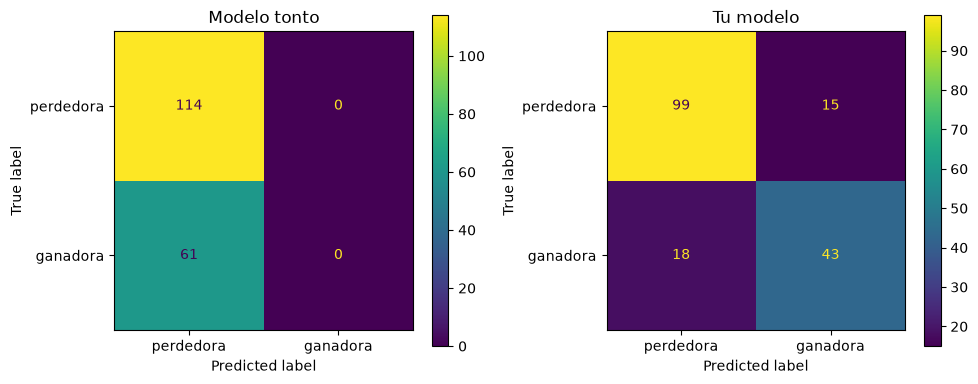
\includegraphics[keepaspectratio]{Copy_of_Laboratorio_4_files/73afac746650ef80dd6b9f6d7480827d618bb56e.png}}

\protect\phantomsection\label{e776c7ad}
\begin{quote}
\textbf{Responde aquí:} compara la exactitud y el F1 de los dos modelos.
¿Qué hace mal el modelo tonto que mirar únicamente la exactitud podría
ocultar?
\end{quote}

\textbf{Respuesta:} El modelo tonto solo predice la clase "false", no va
a poder ver la temporada ganadora porque jamás predice "True". Su
exactitud es solo el porcentaje de datos falsos, y su recall es cero.

\textbf{Exactitud:} el modelo tonto saca 0.651, el modelo real 0.811 ---
una mejora de 16 puntos. \textbf{F1:} el modelo tonto saca 0.000, el
modelo real 0.723 --- ahí la diferencia es total, no incremental.

Esa brecha en el F1 revela lo que la exactitud esconde: el modelo tonto
es tuerto, nunca predice \texttt{True} (siempre responde \texttt{False},
la clase más frecuente), así que su recall sobre
\texttt{ganadora\ =\ True} es 0 --- no detecta ni una sola temporada
ganadora. Aun así, como el 65 \% de las temporadas son \texttt{False},
acertar por pura repetición ya le da 0.651 de exactitud. Mirando solo la
exactitud, 0.651 no parece un desastre; el F1 en 0 deja claro que el
modelo tonto \textbf{ignora por completo la clase que nos interesa
detectar}.

\textbf{Recomendación} Será interesante probar con un modelo que
responda al azar en binomial con un porcentaje de aciertos determinado y
hacer varias corridas.

\protect\phantomsection\label{89ad06f0}
\begin{center}\rule{0.5\linewidth}{0.5pt}\end{center}

\subsection{6 · Sacarlo de tu
computadora}\label{6--sacarlo-de-tu-computadora}

Hasta aquí solo había que ejecutar. \textbf{Esta parte sí la levantas
tú.}

Guardamos el \textbf{Pipeline completo} (escalador + modelo). Si
guardaras solo la regresión logística, la API recibiría datos sin
escalar y devolvería disparates \textbf{sin lanzar ningún error}.

\protect\phantomsection\label{37580302}
\begin{Shaded}
\begin{Highlighting}[]
\ImportTok{import}\NormalTok{ joblib, pathlib}

\NormalTok{pathlib.Path(}\StringTok{"modelos"}\NormalTok{).mkdir(exist\_ok}\OperatorTok{=}\VariableTok{True}\NormalTok{)}
\NormalTok{joblib.dump(modelo, }\StringTok{"modelos/modelo.joblib"}\NormalTok{)     }\CommentTok{\# el Pipeline ENTERO}
\BuiltInTok{print}\NormalTok{(}\StringTok{"modelos/modelo.joblib guardado"}\NormalTok{)}
\end{Highlighting}
\end{Shaded}

\begin{verbatim}
modelos/modelo.joblib guardado
\end{verbatim}

\protect\phantomsection\label{6fffec23}
Estos dos archivos los necesita Docker:

\protect\phantomsection\label{70e31cdf}
\begin{Shaded}
\begin{Highlighting}[]
\NormalTok{servir }\OperatorTok{=}\NormalTok{ [}
    \StringTok{"import joblib"}\NormalTok{,}
    \StringTok{"from fastapi import FastAPI"}\NormalTok{,}
    \StringTok{""}\NormalTok{,}
    \StringTok{\textquotesingle{}modelo = joblib.load("modelos/modelo.joblib")\textquotesingle{}}\NormalTok{,}
    \StringTok{\textquotesingle{}app = FastAPI(title="Temporada ganadora")\textquotesingle{}}\NormalTok{,}
    \StringTok{""}\NormalTok{,}
    \StringTok{\textquotesingle{}@app.get("/predecir")\textquotesingle{}}\NormalTok{,}
    \StringTok{"def predecir(gf: int, ga: int):"}\NormalTok{,}
    \StringTok{"    x = [[gf, ga, gf {-} ga]]"}\NormalTok{,}
    \StringTok{\textquotesingle{}    return \{"ganadora": bool(modelo.predict(x)[0]),\textquotesingle{}}\NormalTok{,}
    \StringTok{\textquotesingle{}            "probabilidad": round(float(modelo.predict\_proba(x)[0][1]), 3)\}\textquotesingle{}}\NormalTok{,}
\NormalTok{]}

\NormalTok{imagen }\OperatorTok{=}\NormalTok{ [}
    \StringTok{"FROM python:3.12{-}slim"}\NormalTok{,}
    \StringTok{"WORKDIR /app"}\NormalTok{,}
    \StringTok{"RUN pip install {-}{-}no{-}cache{-}dir fastapi uvicorn scikit{-}learn joblib"}\NormalTok{,}
    \StringTok{"COPY servir.py ."}\NormalTok{,}
    \StringTok{\textquotesingle{}CMD ["uvicorn", "servir:app", "{-}{-}host", "0.0.0.0", "{-}{-}port", "8000"]\textquotesingle{}}\NormalTok{,}
\NormalTok{]}

\BuiltInTok{open}\NormalTok{(}\StringTok{"servir.py"}\NormalTok{, }\StringTok{"w"}\NormalTok{, encoding}\OperatorTok{=}\StringTok{"utf{-}8"}\NormalTok{).write(}\StringTok{"}\CharTok{\textbackslash{}n}\StringTok{"}\NormalTok{.join(servir))}
\BuiltInTok{open}\NormalTok{(}\StringTok{"Dockerfile"}\NormalTok{, }\StringTok{"w"}\NormalTok{, encoding}\OperatorTok{=}\StringTok{"utf{-}8"}\NormalTok{).write(}\StringTok{"}\CharTok{\textbackslash{}n}\StringTok{"}\NormalTok{.join(imagen))}
\BuiltInTok{print}\NormalTok{(}\StringTok{"servir.py y Dockerfile escritos"}\NormalTok{)}
\end{Highlighting}
\end{Shaded}

\begin{verbatim}
servir.py y Dockerfile escritos
\end{verbatim}

\protect\phantomsection\label{e222cd91}
En la \textbf{terminal}, dentro de esta carpeta:

\begin{Shaded}
\begin{Highlighting}[]
\ExtensionTok{docker}\NormalTok{ build }\AttributeTok{{-}t}\NormalTok{ nhl{-}api .}
\ExtensionTok{docker}\NormalTok{ run }\AttributeTok{{-}p}\NormalTok{ 8000:8000 }\AttributeTok{{-}v} \StringTok{"}\VariableTok{$\{PWD\}}\StringTok{/modelos:/app/modelos"}\NormalTok{ nhl{-}api}
\end{Highlighting}
\end{Shaded}

Abre \textbf{\url{http://localhost:8000/docs}}, prueba
\texttt{/predecir} con \texttt{gf=300} y \texttt{ga=250}, y captura la
respuesta.

\begin{itemize}
\tightlist
\item
  \texttt{-p\ 8000:8000} conecta el puerto del contenedor con el de tu
  máquina
\item
  \texttt{-v\ ...} mete tu carpeta \texttt{modelos/} dentro del
  contenedor
\end{itemize}

\begin{quote}
\textbf{Prueba esto:} corre el contenedor \textbf{sin} el \texttt{-v}.
¿Qué pasa y por qué?
\end{quote}

\protect\phantomsection\label{d6d0270a}
\begin{center}\rule{0.5\linewidth}{0.5pt}\end{center}

\subsection{Entrega}\label{entrega}

En una celda de texto al final del notebook:

\begin{enumerate}
\tightlist
\item
  La exactitud y el F1 del \textbf{modelo tonto} y de \textbf{tu
  modelo}.
\item
  Qué hace mal el modelo tonto que la exactitud no deja ver.
\item
  Por qué se guarda el \textbf{Pipeline completo}
  (\texttt{StandardScaler} + \texttt{LogisticRegression}) y no solo la
  regresión logística.
\item
  Qué pasó al correr el contenedor \textbf{sin} \texttt{-v}.
\end{enumerate}

Y la \textbf{captura de la API respondiendo} en
\texttt{http://localhost:8000/docs}.

\begin{center}\rule{0.5\linewidth}{0.5pt}\end{center}

\begin{quote}
\textbf{Si haces la parte 7 (opcional)}, añade además:

\begin{itemize}
\tightlist
\item
  la \textbf{URL pública} de tu API
\item
  una captura de
  \texttt{https://\textless{}tu-dominio\textgreater{}/docs} con una
  llamada a \texttt{/predecir} que haya respondido bien
\end{itemize}
\end{quote}

\protect\phantomsection\label{056808de}
\begin{center}\rule{0.5\linewidth}{0.5pt}\end{center}

\section{7 · Del localhost a Internet ·
OPCIONAL}\label{7--del-localhost-a-internet--opcional}

\begin{quote}
\textbf{Esta parte no es obligatoria.} El laboratorio ya está completo
con la entrega de arriba. Lo que sigue es para quien quiera dar el
último paso: que la API deje de vivir en tu computadora y quede
publicada en Internet, con una dirección que pueda abrir cualquiera.

Necesitas una cuenta de GitHub y unos 25 minutos.
\end{quote}

Tu API funciona\ldots{} \textbf{solo en tu computadora}. Eso es lo que
significa \texttt{localhost}: «esta misma máquina». Si cierras la
laptop, se acabó; y nadie más puede abrirla.

\begin{verbatim}
ANTES

Navegador (el tuyo)
     ↓
localhost:8000
     ↓
Contenedor Docker
     ↓
FastAPI
     ↓
modelo.joblib
\end{verbatim}

\begin{verbatim}
AHORA

Navegador de cualquier persona
          ↓
       Internet
          ↓
  servidor en la nube
          ↓
   Contenedor Docker
          ↓
       FastAPI
          ↓
    modelo.joblib
\end{verbatim}

Vamos a subir \textbf{el mismo contenedor} a un servidor en la nube y
obtener una URL pública. Usaremos \textbf{Railway}, porque construye la
aplicación a partir del \texttt{Dockerfile} que ya tienes: no hay que
aprender nada nuevo.

\begin{verbatim}
Proyecto local  →  GitHub  →  Railway  →  Dockerfile  →  contenedor  →  URL pública
\end{verbatim}

\protect\phantomsection\label{4678b3c6}
\subsubsection{Primero: que el modelo viaje dentro de la
imagen}\label{primero-que-el-modelo-viaje-dentro-de-la-imagen}

En local, el modelo entraba al contenedor \textbf{desde tu carpeta}, con
\texttt{-v}:

\begin{verbatim}
TU COMPUTADORA              CONTENEDOR
modelos/                    /app/modelos/
└── modelo.joblib    -v →   └── modelo.joblib
\end{verbatim}

Pero en la nube \textbf{no existe tu carpeta}. El servidor no tiene un
\texttt{modelos/} que montar. Así que cambiamos la estrategia: metemos
el modelo \textbf{dentro de la imagen} al construirla.

\begin{verbatim}
modelo.joblib  →  docker build  →  queda dentro de la imagen
\end{verbatim}

Eso no significa que el \texttt{-v} estuviera mal. Son \textbf{dos
formas distintas} de hacer que un archivo esté disponible dentro de un
contenedor: montarlo desde fuera, o copiarlo adentro.

\protect\phantomsection\label{aa25d645}
\begin{Shaded}
\begin{Highlighting}[]
\NormalTok{imagen\_nube }\OperatorTok{=}\NormalTok{ [}
    \StringTok{"FROM python:3.12{-}slim"}\NormalTok{,}
    \StringTok{"WORKDIR /app"}\NormalTok{,}
    \StringTok{"RUN pip install {-}{-}no{-}cache{-}dir fastapi uvicorn scikit{-}learn joblib"}\NormalTok{,}
    \StringTok{"COPY servir.py ."}\NormalTok{,}
    \StringTok{"COPY modelos ./modelos"}\NormalTok{,                      }\CommentTok{\# ← el modelo entra a la imagen}
    \StringTok{\textquotesingle{}CMD ["sh", "{-}c", "uvicorn servir:app {-}{-}host 0.0.0.0 {-}{-}port $}\SpecialCharTok{\{PORT:{-}8000\}}\StringTok{"]\textquotesingle{}}\NormalTok{,}
\NormalTok{]}

\BuiltInTok{open}\NormalTok{(}\StringTok{"Dockerfile"}\NormalTok{, }\StringTok{"w"}\NormalTok{, encoding}\OperatorTok{=}\StringTok{"utf{-}8"}\NormalTok{).write(}\StringTok{"}\CharTok{\textbackslash{}n}\StringTok{"}\NormalTok{.join(imagen\_nube))}
\BuiltInTok{print}\NormalTok{(}\StringTok{"Dockerfile actualizado para la nube"}\NormalTok{)}
\BuiltInTok{print}\NormalTok{()}
\BuiltInTok{print}\NormalTok{(}\BuiltInTok{open}\NormalTok{(}\StringTok{"Dockerfile"}\NormalTok{, encoding}\OperatorTok{=}\StringTok{"utf{-}8"}\NormalTok{).read())}
\end{Highlighting}
\end{Shaded}

\begin{verbatim}
Dockerfile actualizado para la nube

FROM python:3.12-slim
WORKDIR /app
RUN pip install --no-cache-dir fastapi uvicorn scikit-learn joblib
COPY servir.py .
COPY modelos ./modelos
CMD ["sh", "-c", "uvicorn servir:app --host 0.0.0.0 --port ${PORT:-8000}"]
\end{verbatim}

\protect\phantomsection\label{5eece350}
Dos líneas nuevas:

\textbf{\texttt{COPY\ modelos\ ./modelos}} --- copia tu carpeta
\texttt{modelos/} (con el \texttt{.joblib} dentro) a la imagen. Ya no
hace falta \texttt{-v}.

\textbf{\texttt{-\/-port\ \$\{PORT:-8000\}}} --- así se lee:

\begin{verbatim}
¿existe una variable PORT?
   sí  →  usa ese puerto
   no  →  usa 8000
\end{verbatim}

En tu computadora \texttt{PORT} no está definido, así que sigue siendo
el 8000 de siempre. En la nube, \textbf{la plataforma decide el puerto}
y te lo pasa en esa variable. Con esto el mismo Dockerfile sirve en los
dos sitios.

\protect\phantomsection\label{574ee7b8}
\subsubsection{Subir el proyecto a
GitHub}\label{subir-el-proyecto-a-github}

Railway lee tu código desde GitHub. En el repositorio tienen que estar,
como mínimo, estos tres:

\begin{verbatim}
Dockerfile
servir.py
modelos/modelo.joblib
\end{verbatim}

Desde la terminal, en la carpeta del proyecto:

\begin{Shaded}
\begin{Highlighting}[]
\FunctionTok{git}\NormalTok{ add .}
\FunctionTok{git}\NormalTok{ commit }\AttributeTok{{-}m} \StringTok{"Deploy NHL API"}
\FunctionTok{git}\NormalTok{ push}
\end{Highlighting}
\end{Shaded}

Si aún no tienes repositorio, créalo en GitHub y sigue las instrucciones
que la propia página te muestra al crearlo.

\begin{quote}
\textbf{Ojo:} si tienes un \texttt{.gitignore} que ignora
\texttt{*.joblib} o la carpeta \texttt{modelos/}, el modelo \textbf{no
se sube} y el despliegue falla. Comprueba con \texttt{git\ status} que
el \texttt{.joblib} aparece entre los archivos añadidos.
\end{quote}

\protect\phantomsection\label{f314cfa5}
\begin{quote}
\textbf{Si haces la parte 7 (opcional)}, añade además:

\begin{itemize}
\tightlist
\item
  la \textbf{URL pública} de tu API
\end{itemize}
\end{quote}

\subsubsection{Desplegar en Railway}\label{desplegar-en-railway}

El flujo, sin depender de cómo se llamen los botones hoy:

\begin{enumerate}
\tightlist
\item
  Entra a \textbf{Railway} y crea una cuenta (puedes usar la de GitHub).
\item
  Crea un \textbf{proyecto nuevo}.
\item
  Elige desplegar \textbf{desde un repositorio de GitHub}.
\item
  Selecciona el repositorio de este laboratorio.
\item
  Railway detecta el \texttt{Dockerfile} y \textbf{construye la imagen}.
  Tarda unos minutos: está haciendo lo mismo que hizo tu
  \texttt{docker\ build}, pero en su servidor.
\item
  Cuando termina, \textbf{arranca el contenedor}.
\item
  En la configuración del servicio, \textbf{genera un dominio público}.
\item
  Abre esa URL.
\end{enumerate}

Tu dirección será algo parecido a esto (\textbf{es solo un ejemplo, no
la copies}):

\begin{verbatim}
https://mi-nhl-api.up.railway.app/docs
\end{verbatim}

Ahí tienes la misma página \texttt{/docs} que viste en
\texttt{localhost}, pero servida desde Internet. Prueba
\texttt{GET\ /predecir} con \texttt{gf\ =\ 300} y \texttt{ga\ =\ 250}.
Debería responder algo con esta forma:

\begin{Shaded}
\begin{Highlighting}[]
\FunctionTok{\{}
  \DataTypeTok{"ganadora"}\FunctionTok{:} \KeywordTok{true}\FunctionTok{,}
  \DataTypeTok{"probabilidad"}\FunctionTok{:} \FloatTok{0.87}
\FunctionTok{\}}
\end{Highlighting}
\end{Shaded}

El número exacto depende de tu modelo; lo que importa es que responda.

\protect\phantomsection\label{53edd714}
\subsubsection{Qué acabas de
conseguir}\label{quuxe9-acabas-de-conseguir}

\begin{verbatim}
ANTES                        AHORA

Usuario (tú)                 Usuario en Internet
   ↓                                ↓
localhost                       URL pública
   ↓                                ↓
FastAPI                          Railway
   ↓                                ↓
modelo                          contenedor
                                    ↓
                                 FastAPI
                                    ↓
                            Pipeline entrenado
\end{verbatim}

Tu modelo dejó de ser un archivo en tu carpeta y se convirtió en un
\textbf{servicio al que se puede llamar por HTTP}. Cualquier programa
---una app, una página web, otro script--- puede usarlo ahora sin saber
nada de scikit-learn.

{\def\LTcaptype{none} % do not increment counter
\begin{longtable}[]{@{}lll@{}}
\toprule\noalign{}
Etapa & Dirección & Quién puede acceder \\
\midrule\noalign{}
\endhead
\bottomrule\noalign{}
\endlastfoot
Notebook & tu archivo & solo tú \\
FastAPI local & \texttt{localhost:8000} & tu computadora \\
Docker local & \texttt{localhost:8000} & tu computadora \\
Railway & URL HTTPS pública & cualquiera con Internet \\
\end{longtable}
}

Esa última fila es la diferencia entre \textbf{ejecutar} y
\textbf{desplegar}.

\protect\phantomsection\label{jJQmjCPvnYyg}
\subsubsection{Qué acabas de
conseguir}\label{quuxe9-acabas-de-conseguir}

\begin{verbatim}
ANTES                        AHORA

Usuario (tú)                 Usuario en Internet
   ↓                                ↓
localhost                       URL pública
   ↓                                ↓
FastAPI                          Railway
   ↓                                ↓
modelo                          contenedor
                                    ↓
                                 FastAPI
                                    ↓
                            Pipeline entrenado
\end{verbatim}

Tu modelo dejó de ser un archivo en tu carpeta y se convirtió en un
\textbf{servicio al que se puede llamar por HTTP}. Cualquier programa
---una app, una página web, otro script--- puede usarlo ahora sin saber
nada de scikit-learn.

{\def\LTcaptype{none} % do not increment counter
\begin{longtable}[]{@{}lll@{}}
\toprule\noalign{}
Etapa & Dirección & Quién puede acceder \\
\midrule\noalign{}
\endhead
\bottomrule\noalign{}
\endlastfoot
Notebook & tu archivo & solo tú \\
FastAPI local & \texttt{localhost:8000} & tu computadora \\
Docker local & \texttt{localhost:8000} & tu computadora \\
Railway & URL HTTPS pública & cualquiera con Internet \\
\end{longtable}
}

Esa última fila es la diferencia entre \textbf{ejecutar} y
\textbf{desplegar}.

\subsubsection{Parte 7 (opcional)}\label{parte-7-opcional}

Si desplegaste la API, añade también la URL pública y una captura de
\texttt{/predecir} respondiendo correctamente en \texttt{/docs}.

\begin{itemize}
\tightlist
\item
  \textbf{URL pública:} añade aquí tu URL.
\item
  \textbf{Captura:} añade aquí la imagen de la llamada exitosa a
  \texttt{https://\textless{}tu-dominio\textgreater{}/docs}.
\end{itemize}

\protect\phantomsection\label{e0875f6c}
\subsection{Entrega}\label{entrega}

-\/-

\textbf{Entrega:}

\subsubsection{1. Métricas del modelo tonto y de mi
modelo}\label{1-muxe9tricas-del-modelo-tonto-y-de-mi-modelo}

El modelo tonto acierta el 65 \% de los casos, pero sus métricas por
clase muestran que nunca identifica los casos \texttt{True}.

La exactitud y el F1 del \textbf{modelo tonto} exactitud 0.65 y F1 0.79
para False, 0.00 para True. precision recall f1-score support

\begin{verbatim}
   False       0.65      1.00      0.79       114
    True       0.00      0.00      0.00        61

accuracy                           0.65       175
\end{verbatim}

macro avg 0.33 0.50 0.39 175 weighted avg 0.42 0.65 0.51 175

y de

\textbf{tu modelo} exactitud 0.81 y F1 0.86 para False, 0.72 para True.
precision recall f1-score support

\begin{verbatim}
   False       0.85      0.87      0.86       114
    True       0.74      0.70      0.72        61

accuracy                           0.81       175
\end{verbatim}

macro avg 0.79 0.79 0.79 175 weighted avg 0.81 0.81 0.81 175

\subsubsection{2. Qué oculta la exactitud del modelo
tonto}\label{2-quuxe9-oculta-la-exactitud-del-modelo-tonto}

Qué hace mal el modelo tonto que la exactitud no deja ver. El modelo
tonto nunca predice \texttt{True}. Su exactitud parece aceptable porque
la clase \texttt{False} es mayoría en este dataset, pero no detecta
ninguno de los 61 casos \texttt{True} (recall de 0.00).

\subsubsection{3. Por qué guardar el pipeline
completo}\label{3-por-quuxe9-guardar-el-pipeline-completo}

Guardo el pipeline completo (\texttt{StandardScaler} +
\texttt{LogisticRegression}) para poderlo recrear es decir que al cargar
el modelo se apliquen los mismos pasos del flujo de preparación y
predicción que se usaron al entrenarlo.

\subsubsection{\texorpdfstring{4. Qué pasó al ejecutar el contenedor sin
\texttt{-v}}{4. Qué pasó al ejecutar el contenedor sin -v}}\label{4-quuxe9-pasuxf3-al-ejecutar-el-contenedor-sin--v}

No hay la carpeta modelos.

El Dockerfile copia el contenido de la imagen, pero no incluye la
carpeta \texttt{modelos/}. Sin montar esa carpeta, la API no encuentra
\texttt{modelos/modelo.joblib} y falla al iniciar.

\begin{center}\rule{0.5\linewidth}{0.5pt}\end{center}

(.venv)
\href{mailto:paulehmig@Pauls-M4-Max-MacBook-Pro}{\nolinkurl{paulehmig@Pauls-M4-Max-MacBook-Pro}}
Lab04 \% docker run -\/-rm -p 8000:8000 "\$PWD/modelos:/app/modelos"
nhl-api

What\textquotesingle s next: Debug this container error with Gordon →
docker ai "help me fix this container error" docker: invalid reference
format: repository name
(/Users/paulehmig/Documents/Personal/USFQ/MaestriaDataScience/Materias/MSDS\_6005\_Matematicas\_y\_Programacion\_IA/Lab04/modelos)
must be lowercase

Y la \textbf{captura de la API respondiendo} en
\texttt{http://localhost:8000/docs}.

Cuando el contenedor esté corriendo, la documentación interactiva está
en \url{http://localhost:8000/docs}. \textbf{Añade aquí una captura de
la API respondiendo.}

\pandocbounded{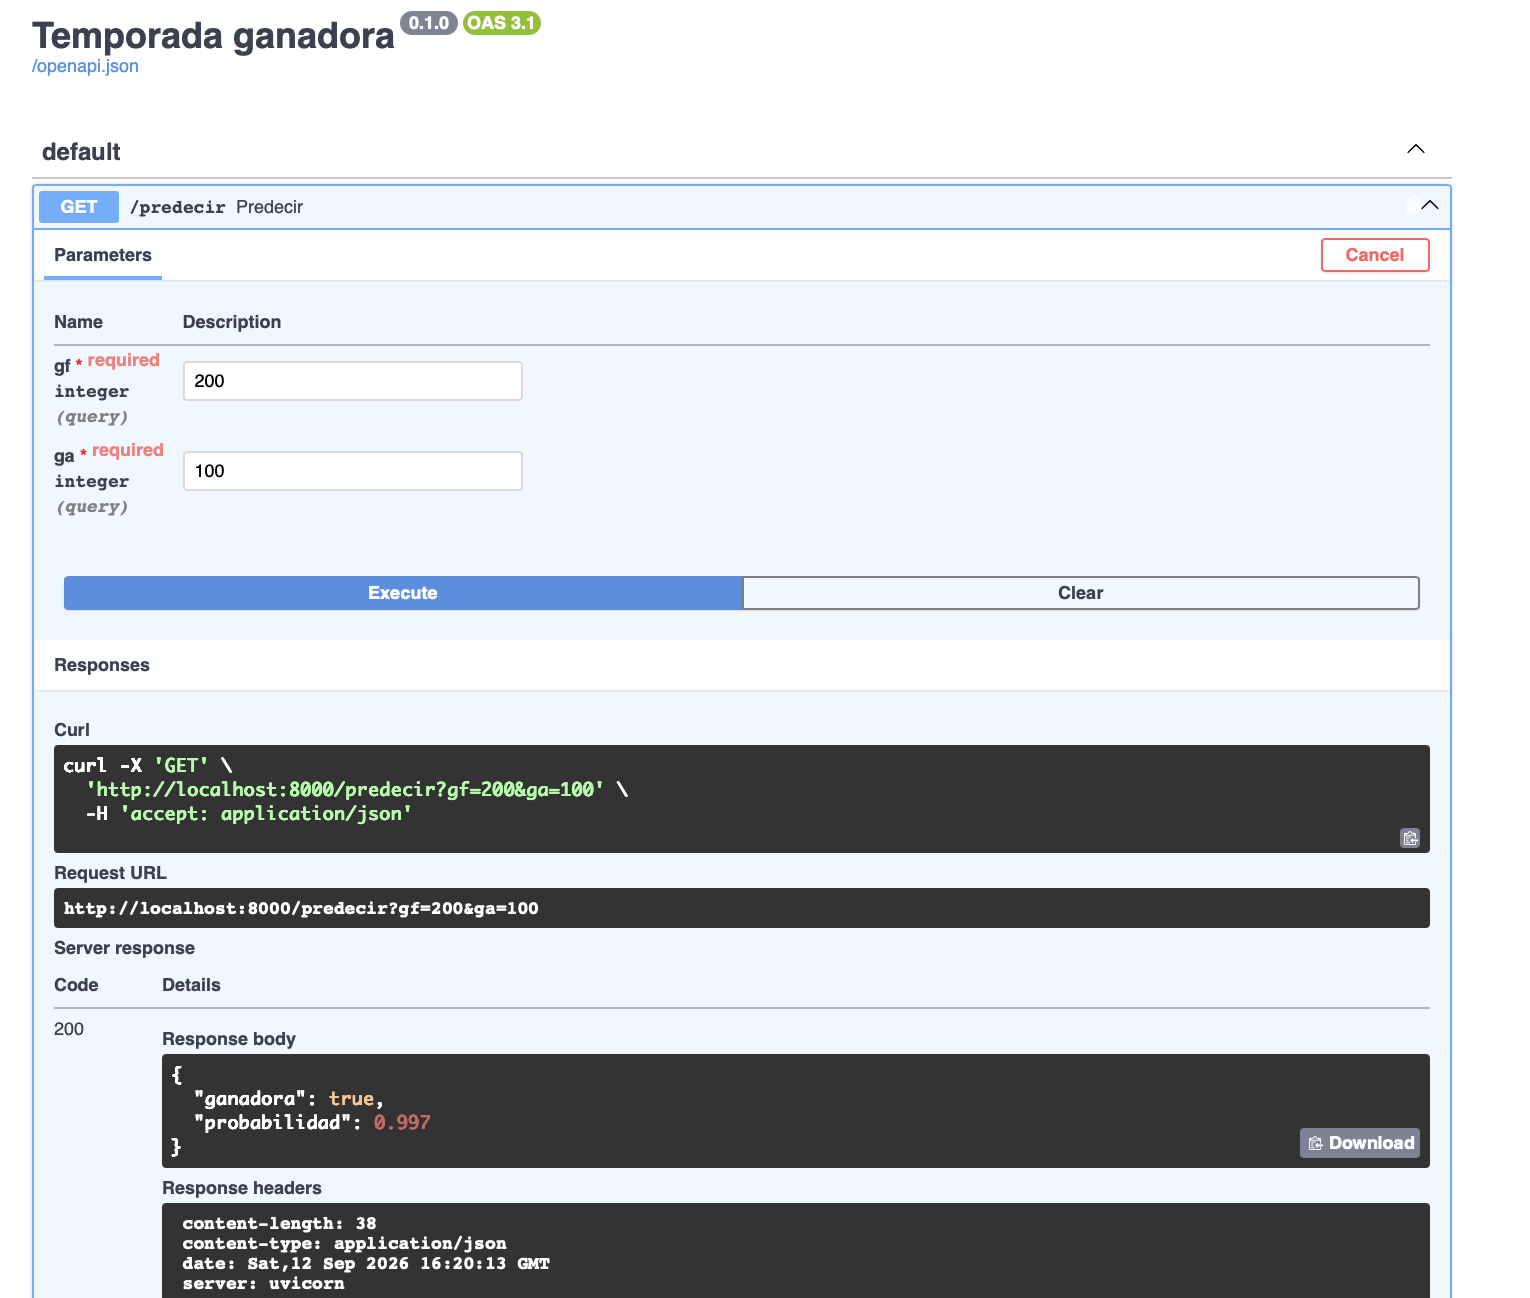
\includegraphics[keepaspectratio,alt={image.png}]{Copy_of_Laboratorio_4_files/e0875f6c-image.png}}

\subsubsection{Parte 7 (opcional)}\label{parte-7-opcional}

\url{https://msds6005lab04-production.up.railway.app/docs}

\begin{quote}
\begin{itemize}
\tightlist
\item
  una captura de
  \texttt{https://msds6005lab04-production.up.railway.app/docs} con una
  llamada a \texttt{/predecir} que haya respondido bien
\end{itemize}
\end{quote}

\pandocbounded{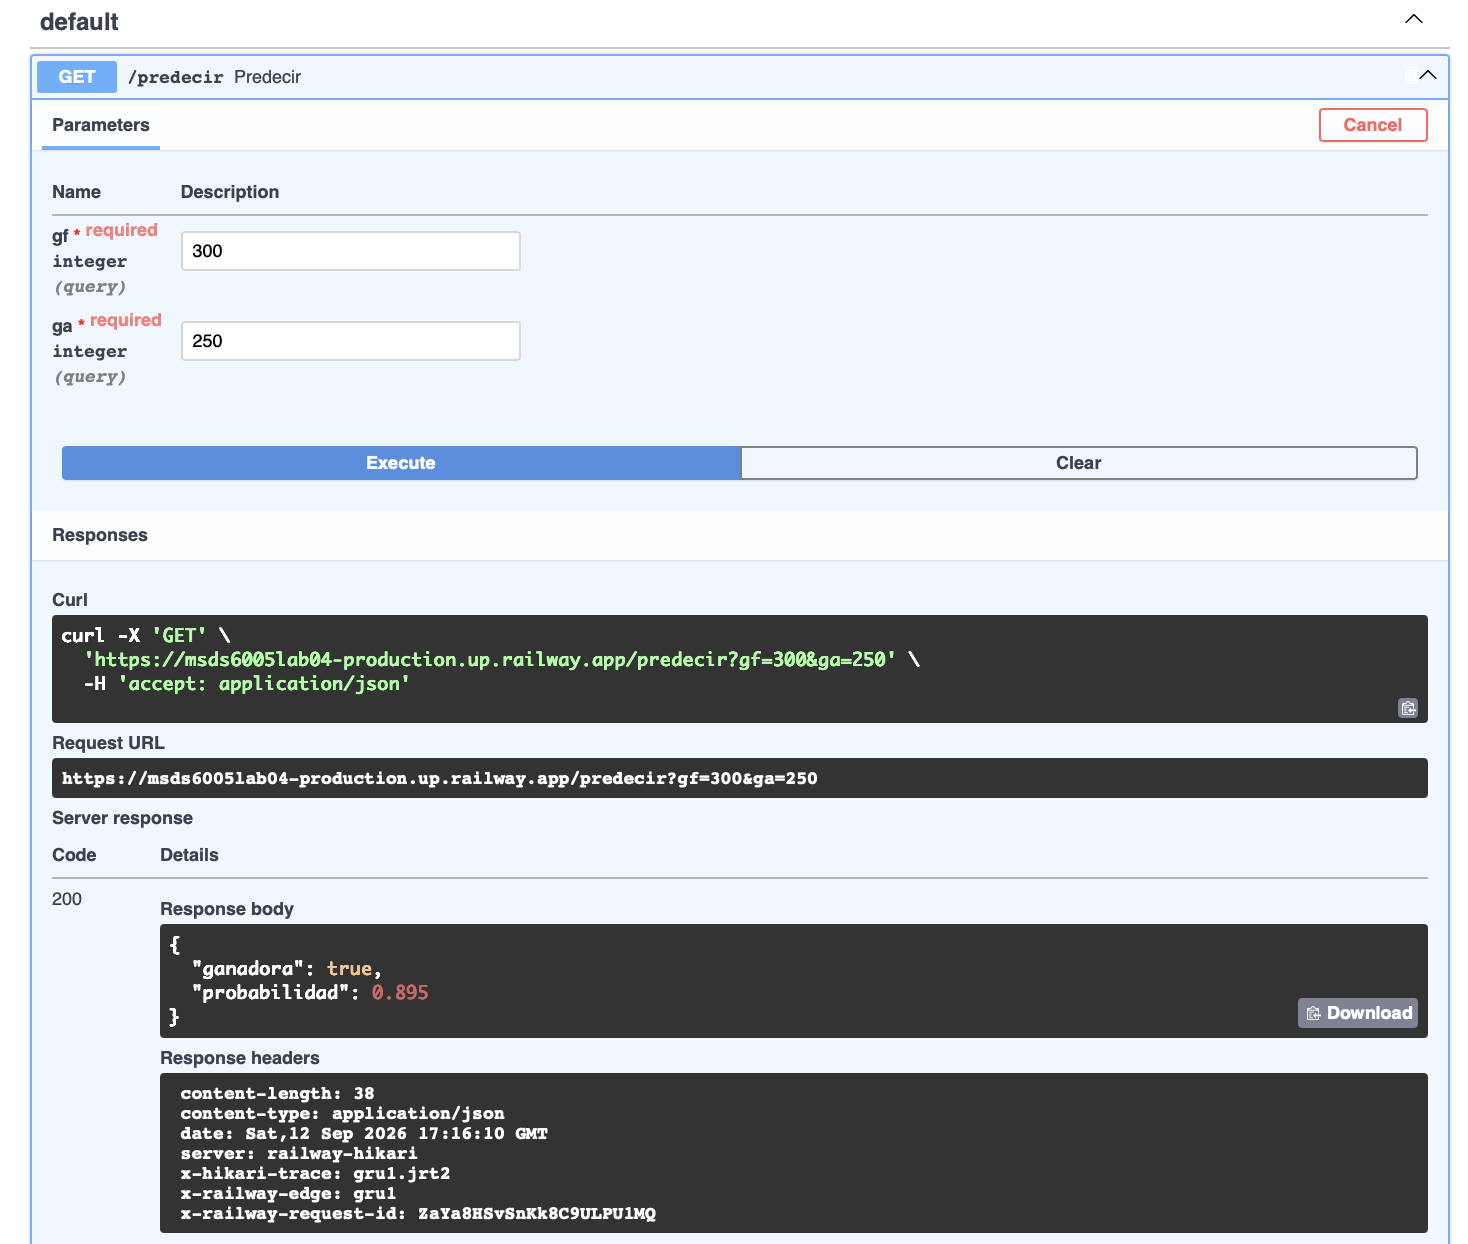
\includegraphics[keepaspectratio,alt={image-2.png}]{Copy_of_Laboratorio_4_files/e0875f6c-image-2.png}}

\end{document}
